    \chapter{Experiments}
        \section{System Architecture}
            The overall work flow of the system for processing from cadastrial map to the 3D model include the key steps as shown in figure~\ref{fig:overall-architecture}.
            \begin{figure}[h]                 
                \centering                 
                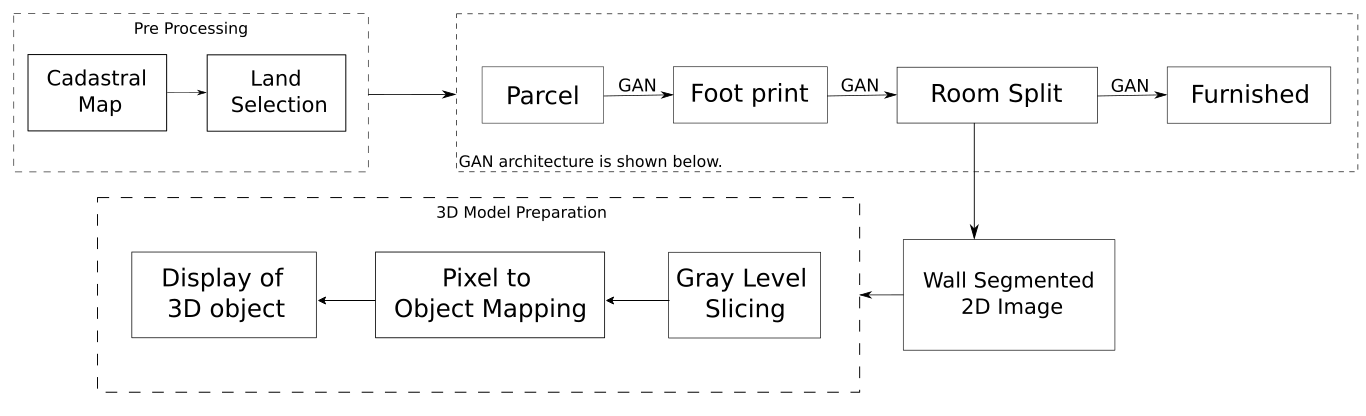
\includegraphics[width=1\textwidth]{img/experiment/overall_architecture.png}                 
                \caption{Overall system's architecture being followed.}                 
                \label{fig:overall-architecture}         
            \end{figure}
            \break
        \section{Color Coding to Dataset}
            We required 5 colors to represent 5 different rooms for room split dataset in ROBIN FP datasets,  other 12 colors to represent 12 different furnitures for furnished dataset and other 1 color to represent windows and doors, altogether 18 different colors other than black and white, which could easily be differenciated without confusion. For this, we used Kelly’s 22 Color of Maximum Contrast.\\
            From the colors of Kelly’s 22 Color,first the exact color code was found out from ISCC-NBS colour system\cite{centore2016srgb} since Kelly's color were standardized using ISCC-NBS number.  Among them first two which are black and white were ignored since black was the color of walls and white was the background. So the next five colors were choosed to represent 5 different rooms. Then next 12 colors were assigned to 12 different furnitures and finally one color was selected to represent doors and window in datasets as shown in table~\ref{tab:colorcode}.\\
            \begin{table}[]
                \caption{Color coding to datasets}
                \label{tab:colorcode}
                \begin{tabular}{|c|c|c|c|}
                    \hline
                    \textbf{Entity} & \textbf{Color} & \textbf{ISCC-NBS No.} & \textbf{Hex Code}\\
                    \hline
                    Bedroom & Yellow & 82 & \#f1bf15\\
                    \hline
                    Bathroom & Purple & 218 & \#9352a8\\
                    \hline
                    Entry & Orange & 48 & \#f7760b\\
                    \hline
                    Kitchen & Light Blue & 180 & \#99c6f9\\
                    \hline
                    Hall & Red & 11 & \#d51c3c\\
                    \hline
                    Arm Chair & Grey & 265 & \#c8b18b\\
                    \hline
                    Bed & Green & 139 & \#23eaa5\\
                    \hline
                    Coffee Table & Purplish Pink & 247 & \#f483cd\\
                    \hline
                    Round Table & Blue & 178 & \#276cbd\\
                    \hline
                    Large Sofa & Yellowish Pink & 26 & \#f59080\\
                    \hline
                    Small Sofa & Voilet & 207 & \#61419c\\
                    \hline
                    Sink & Purplish Red & 255 & \#b83773\\
                    \hline
                    Twin Sink & Greenish Yellow & 97 & \#ebdd21\\
                    \hline
                    Small Sink & Reddish Brown & 40 & \#8b1c0e\\
                    \hline
                    Large Sink & Yellow Green & 115 & \#a7dc26\\
                    \hline
                    Tub & Reddish Orange & 34 & \#e83b1b\\
                    \hline
                    Dinning Table & Olive Green & 126 & \#20340b\\
                    \hline
                    Door & Yellowish Brown & 75 & \#673f0b\\
                    \hline
                    Window & Yellowish Brown & 75 & \#673f0b\\
                    \hline
                \end{tabular}
            \end{table}
            \break
            This way, the colors to represent different entities were standardized. Except this, the border of land area, i.e parcel was drawn of color black for easy creation of following datasets using simple python script.
        \section{Dataset Preparation}\label{section:dataset-preparation}
            We had ROBIN datasets which was a well furnished room layouts for 3 rooms, 4 rooms and 5 rooms. But we needed datasets of parcel, footprint, room split and furnished rooms datasets and each of the segmentation done by color representation. So, we created a python cv2 script with which we can browse all the datasets sequencially and place required parcel lines around the floor plans, place footprint overlay over the original datasets creating footprint datasets, similarly placing overlay of different colors over different rooms giving out room split datasets and placing overlay of different colors over different furniture giving out furnished datasets.\\
            For trainning our GAN models to get required results, we required three different sets of datasets which are paired image datasets in which left image would be the input for the model and the right one be the result that the GAN model need to produce. The three sets of data are:
            \begin{enumerate}[label=\alph*.]
                \item Parcel to Footprint
                \item Footprint to Roomsplit
                \item Roomsplit to Furnished Rooms
            \end{enumerate}
            These are all the paired image datasets as shown in figure~\ref{fig:dataset-final-paired}.
            \begin{figure}[h]
                \centering
                    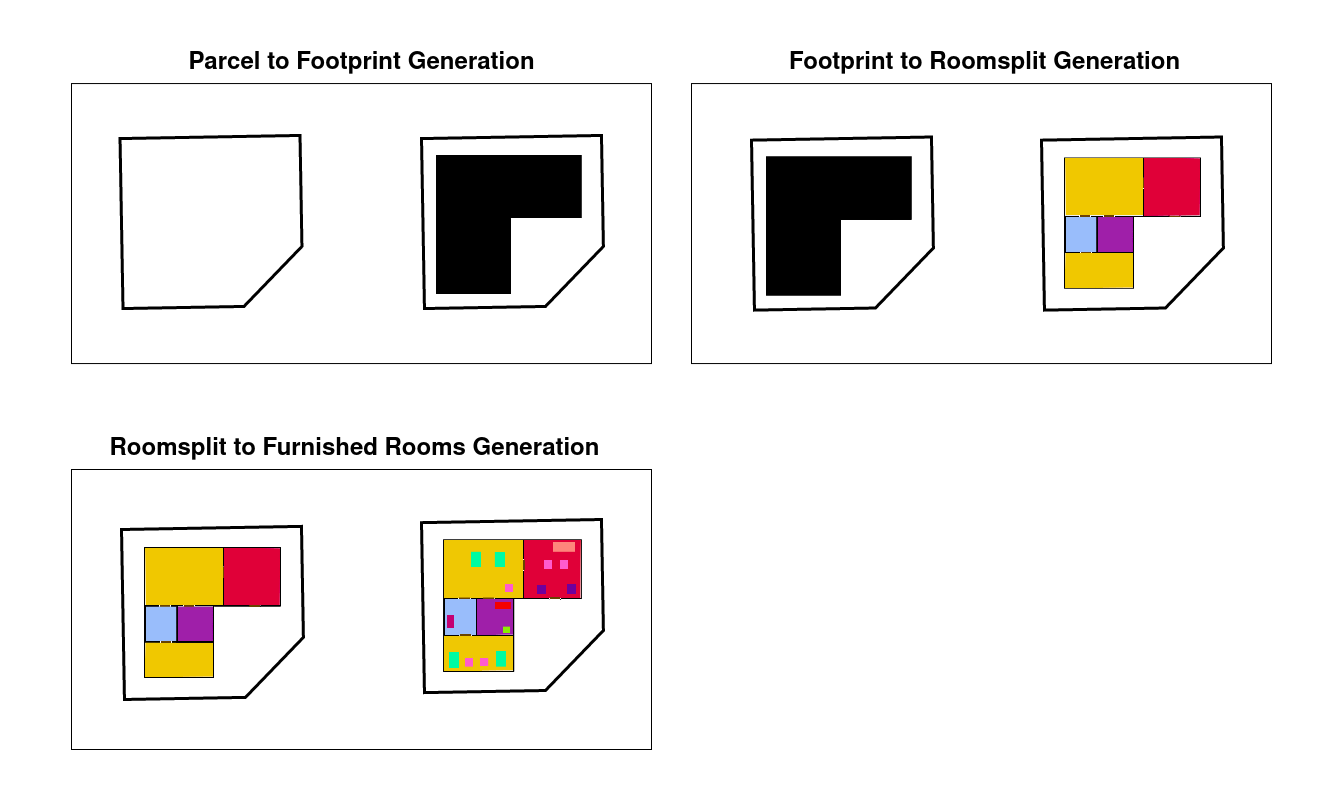
\includegraphics[width=1\linewidth]{img/experiment/dataset/dataset_principal_paired_image.png}
                    \caption{Paired image of parcel and required footprint.}
                    \label{fig:dataset-final-paired}
            \end{figure} 
            To get these paired datasets, we went through steps as in figure~\ref{fig:dataset-final-paired} to prepare the required datasets.
            \begin{figure}[h]
                \centering
                    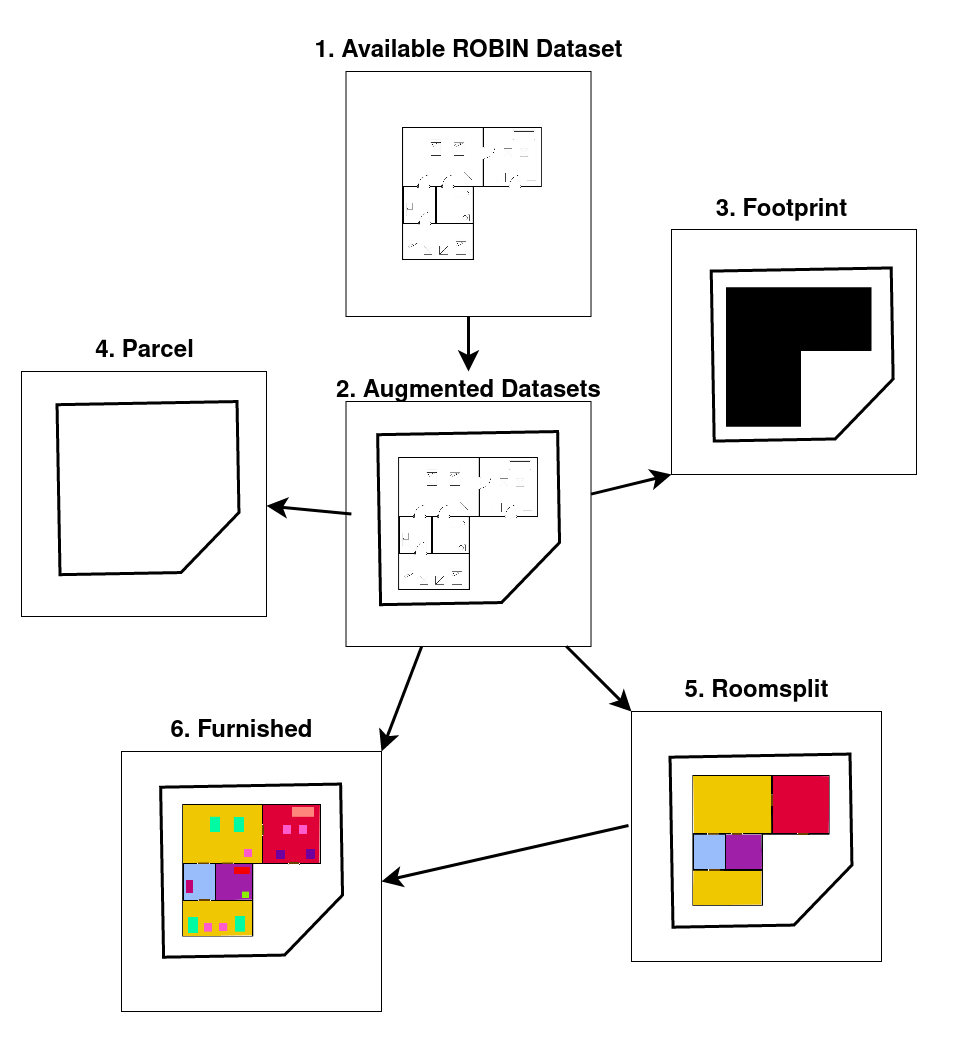
\includegraphics[width=1\linewidth]{img/experiment/dataset/dataset_principal_algorithm.png}
                    \caption{Paired image of parcel and required footprint.}
                    \label{fig:dataset-final-paired}
            \end{figure} 
            
            \subsection{Augmented Dataset Creation}
            In first stage of datasets creation, parcel around the original datasets as shown in figure~\ref{fig:dataset-original}, were placed by creating some enough space around the original floor plans. For this following step were done: First of all the highest width and highest height among all the datasets were found out.  Then the max among the max height and max width were found out which gave us the max size. Then the max size was increased by 25\% and a background image, i.e the foundation size of the datasets was created. This was done to ensure that all the datasets were of same size and not squeezed. Then all the datasets were placed in the square background image and were saved in a separate folder with same name. Also to increase the size of datasets, all the images were again places in the background with slight change in orientation, i.e 30 degree rotation in clockwise direction. This way, the datasets were refined as shown in figure \ref{fig:dataset-augmented}, so as to do some slight process and create other required datasets and the datasets were named as augmented datasets.
            \begin{figure}
                \centering
                \begin{minipage}{.45\textwidth}
                    \centering
                    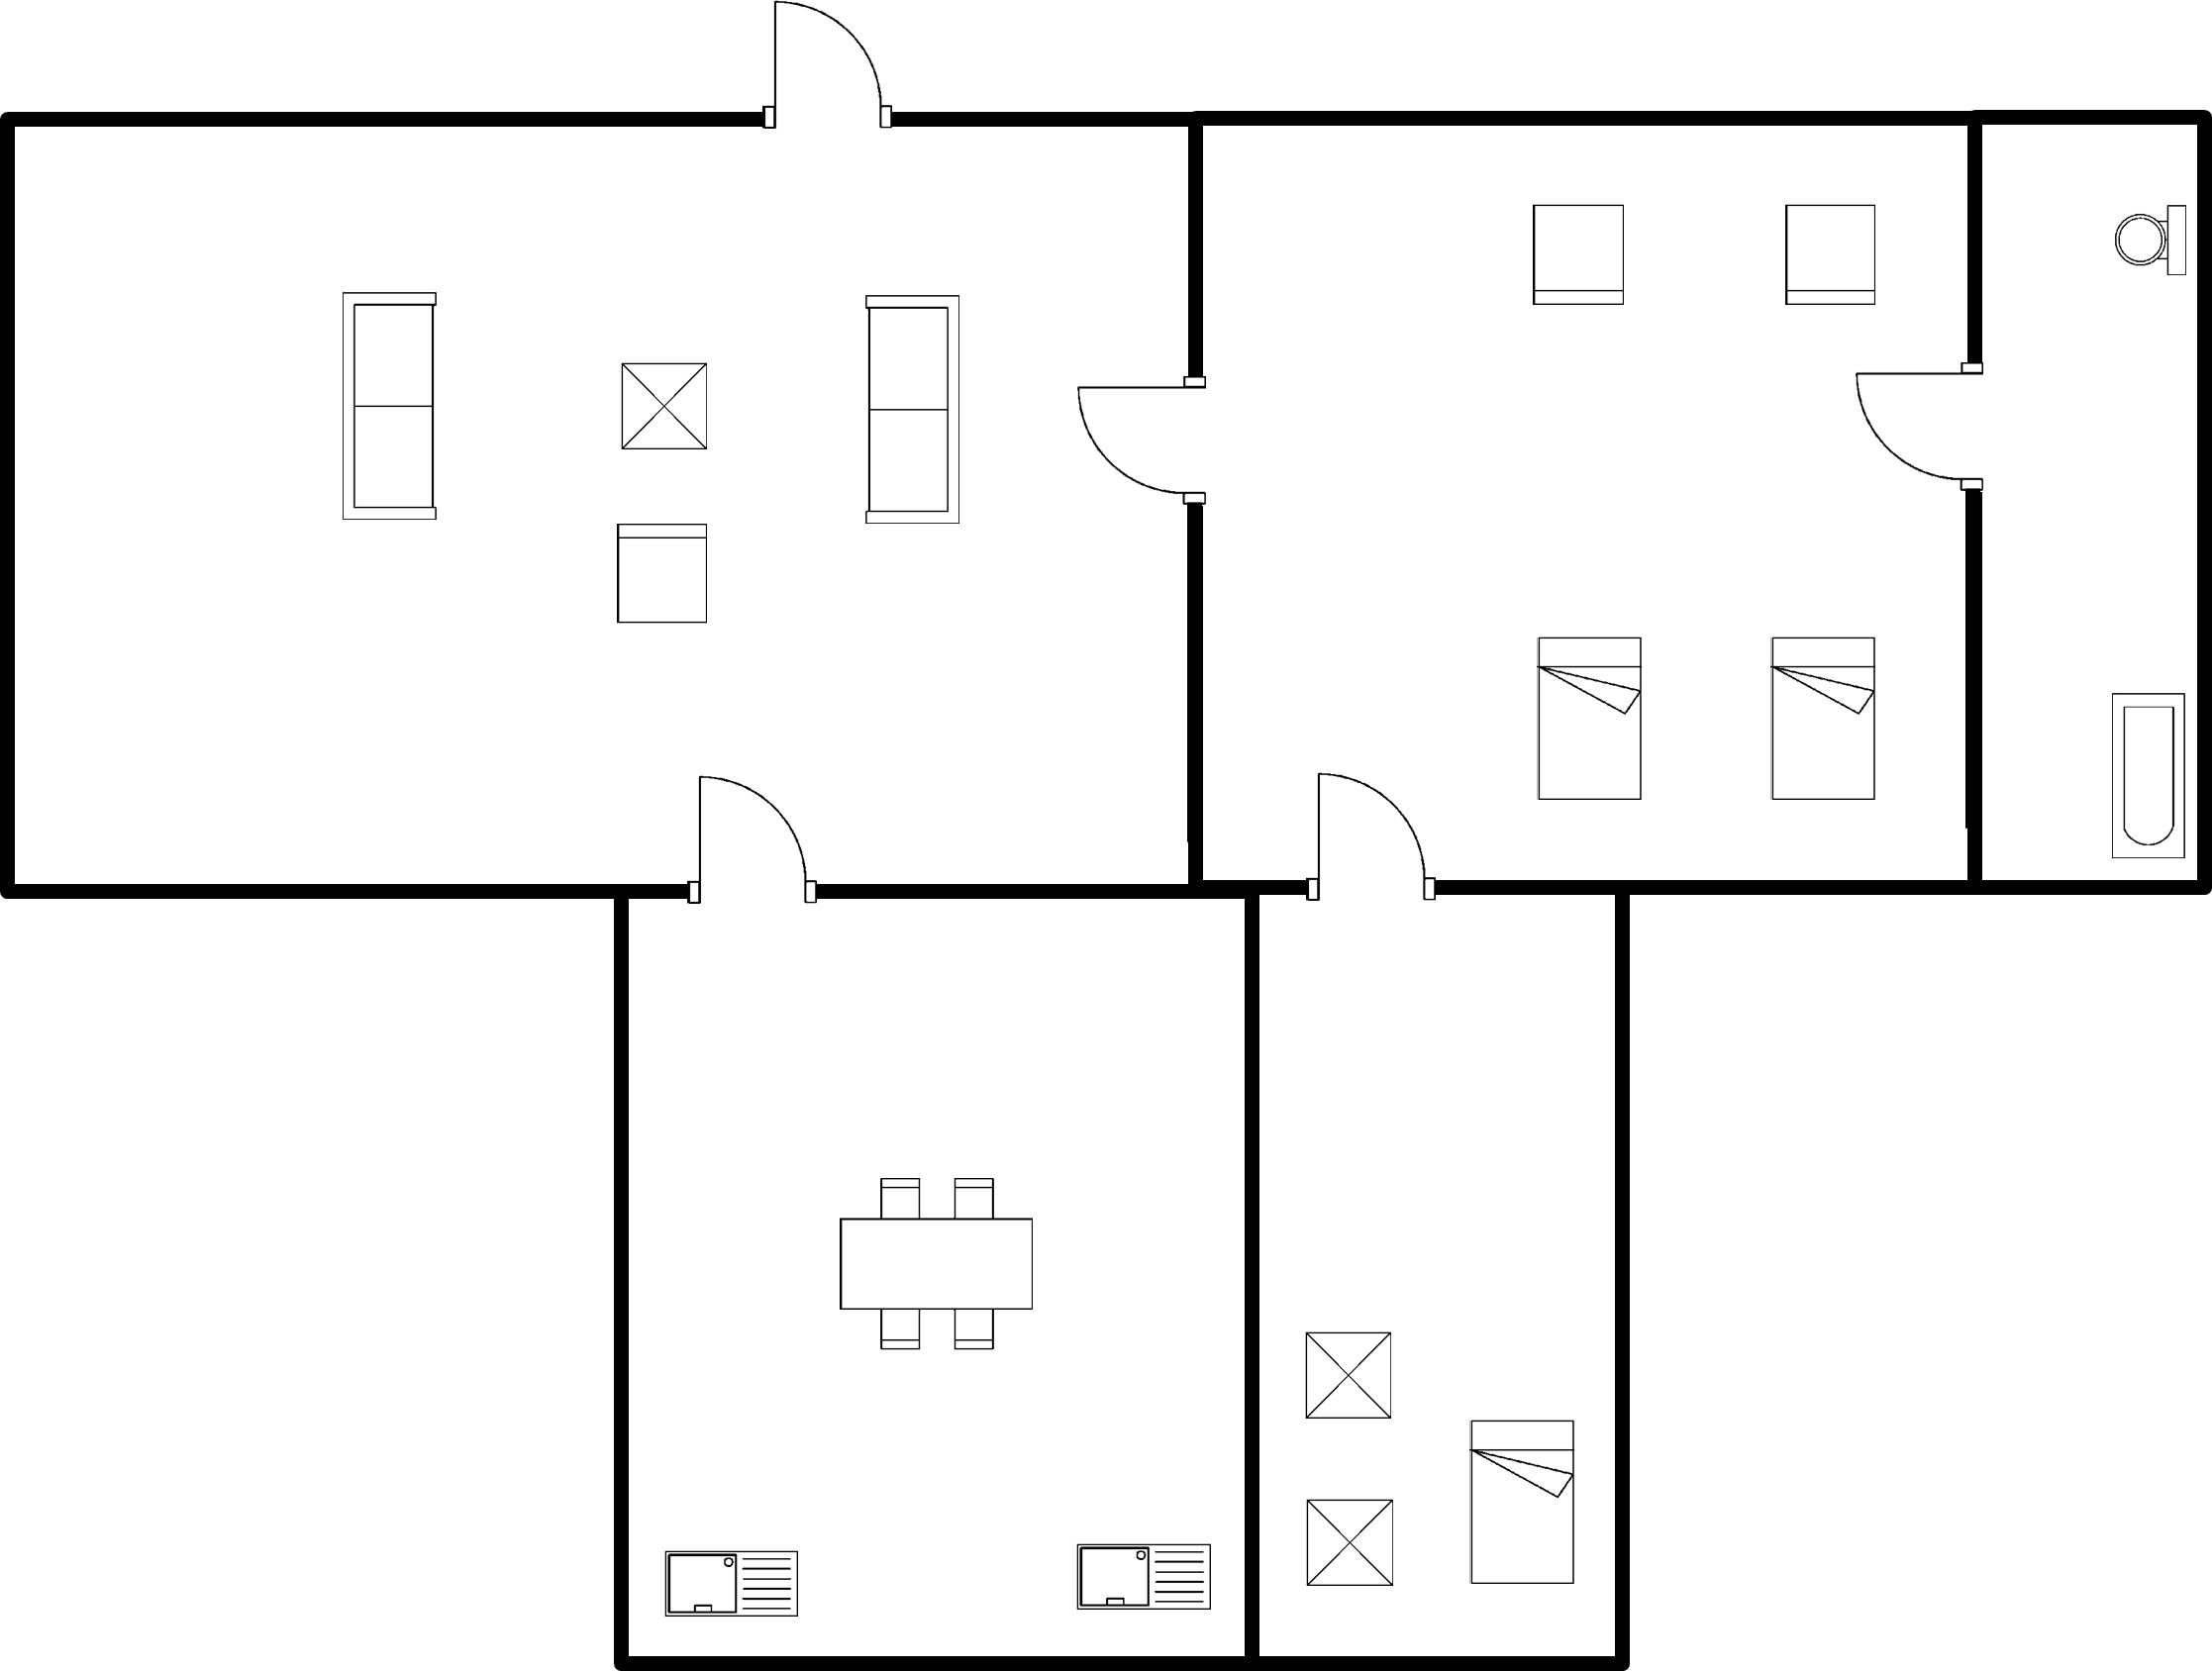
\includegraphics[width=.8\linewidth]{img/experiment/dataset/1a.jpg}
                    \caption{Original dataset from ROBIN Floor Plan datasets.}
                    \label{fig:dataset-original}
                \end{minipage}%
                \hfill
                \begin{minipage}{.45\textwidth}
                    \centering
                    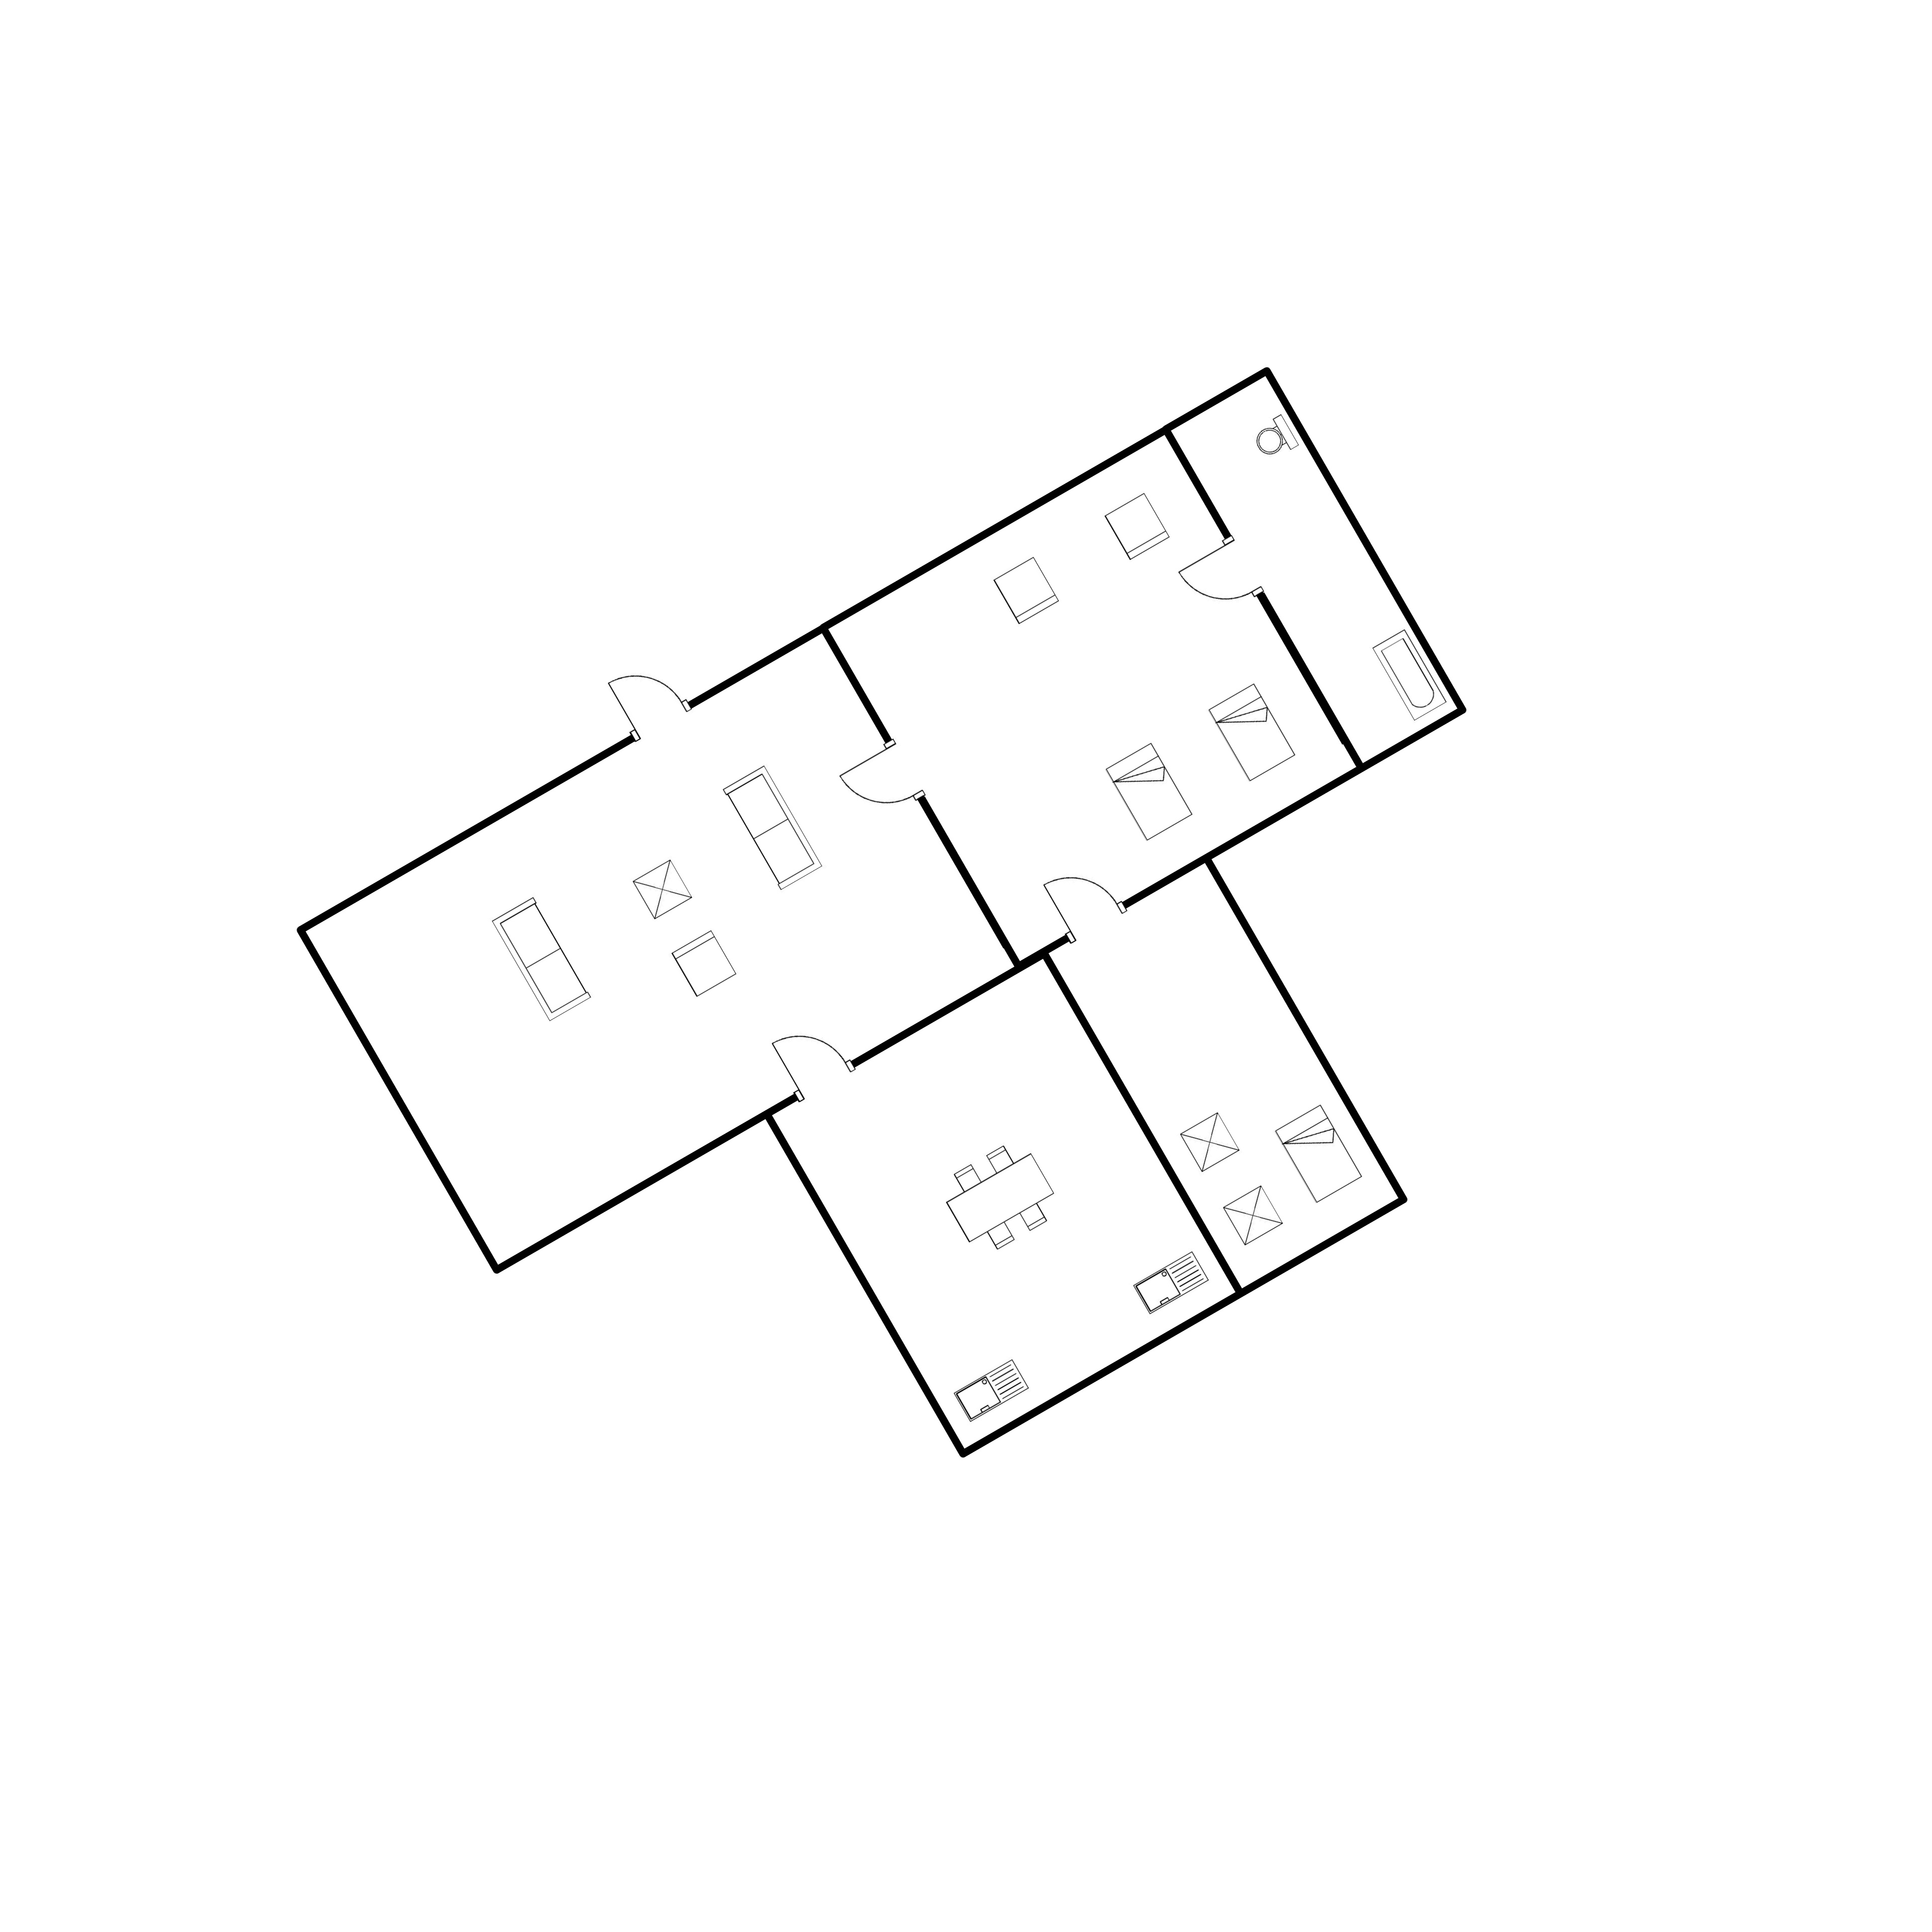
\includegraphics[width=.8\linewidth,frame]{img/experiment/dataset/1b.jpg}
                    \caption{Augmented Dataset with padding and 30 degree clockwise rotation placed in a square frame, resized to 512*512.}
                    \label{fig:dataset-augmented}
                \end{minipage}
            \end{figure}
            \subsection{Parcel and Footprint Generation}
            After getting the augmented datasets, border of the land around the floor plans were drawn manually by loading the datasets sequencially using python cv2 script and we saved  the floor plans with border around them, for further processing and the datasets were labelled as final datasets as in figure \ref{fig:dataset-final}.
            \begin{figure}[h]
                \centering
                \begin{minipage}{.45\textwidth}
                    \centering
                    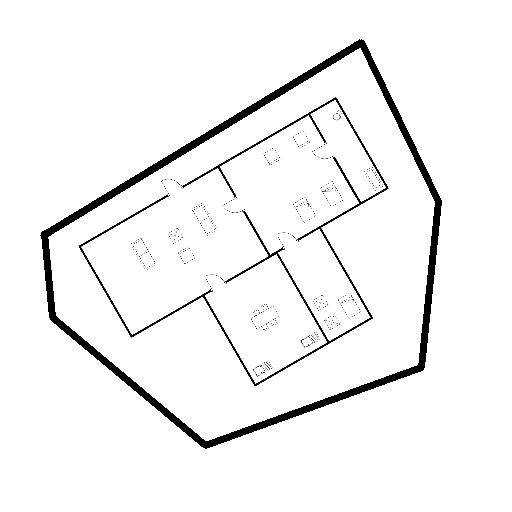
\includegraphics[width=.8\linewidth,frame]{img/experiment/dataset/1final.jpg}
                    \caption{Dataset with border area around.}
                    \label{fig:dataset-final}
                \end{minipage}%
                \hfill
                \begin{minipage}{.45\textwidth}
                    \centering
                    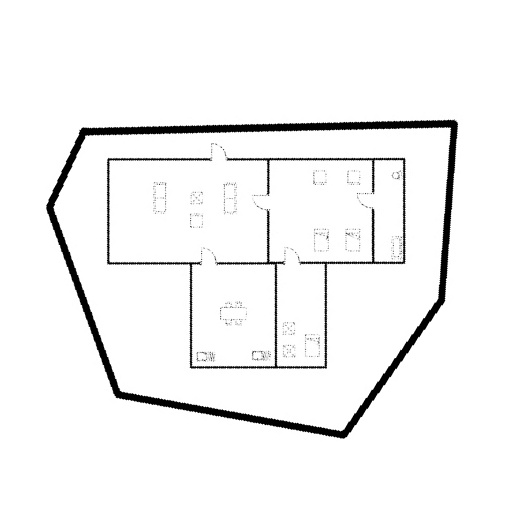
\includegraphics[width=.8\linewidth,frame]{img/experiment/dataset/2final_rotated.jpg}
                    \caption{Final dataset rotated back to normal for further operation of dilation and erosin.}
                    \label{fig:dataset-final-rotated}
                \end{minipage}
            \end{figure}
            \break
            For generation of footprint, we had a python cv2 script to draw a black colored overlay over the floor plan giving us the footprint datasets but it was quite tedious job to do so many datasets manually. So we came up with a image processing tool using dilation and erosion. Dilation would increase the width of any lines or pixels in the image and erosion would decrease the width of the lines or pixels in the image.  Using this concept we created footprint by following method:
            First the image was rotated 30 degree anticlockwise as shown in figure~\ref{fig:dataset-final-rotated} if it was rotated once before which was identified using the naming convention and then dilated with 5*5 pixels which would increase the width of white parts of the image as in figure~\ref{fig:dataset-final-dilated}, resulting in decrease of width of the black lines. The lines with width less than 5 pixel would disappear in this step.Then again erosion with 5*5 stride size is done which would bring back the previous image as shown in figure~\ref{fig:dataset-final-eroded}, except the thin lines that disappeared during dilation would not come back again.This step would clean the floor plans and gives clean parcel.\\
            \begin{figure}[h]
                \centering
                \begin{minipage}{.45\textwidth}
                    \centering
                    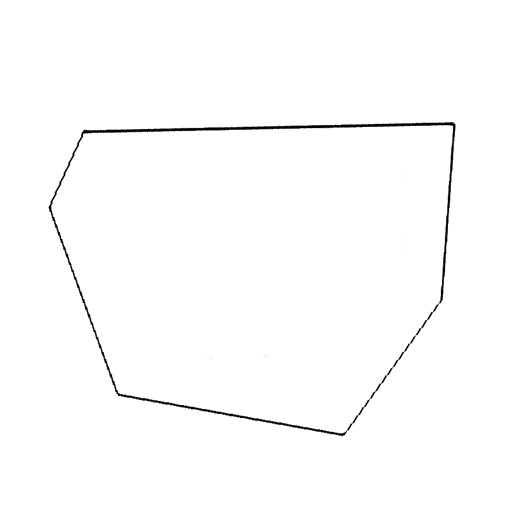
\includegraphics[width=.8\linewidth,frame]{img/experiment/dataset/3dilate_img.jpg}
                    \caption{Result when rotated final image is dilated by stride of 5*5.}
                    \label{fig:dataset-final-dilated}
                \end{minipage}%
                \hfill
                \begin{minipage}{.45\textwidth}
                    \centering
                    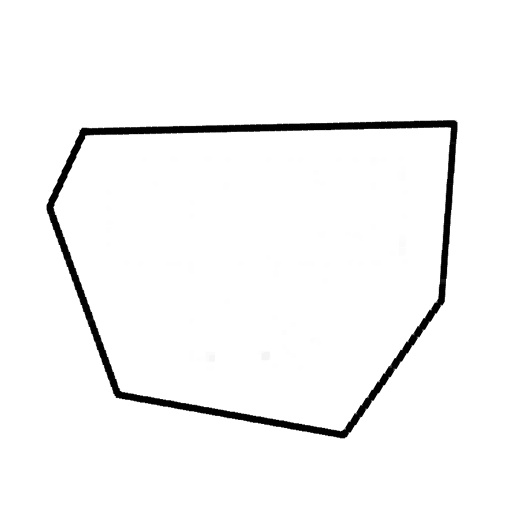
\includegraphics[width=.8\linewidth,frame]{img/experiment/dataset/4erode_img.jpg}
                    \caption{Result when dilated image is eroded by stride of 5*5.}
                    \label{fig:dataset-final-eroded}
                \end{minipage}
            \end{figure}    
            \break
            If required, the parcel is rotated agian by 30 degree clockwise to get the require parcel image of the final image as in figure~\ref{fig:dataset-final-parcel}.\\
            \begin{figure}[h]
                \centering
                \begin{minipage}{.5\textwidth}
                    \centering
                    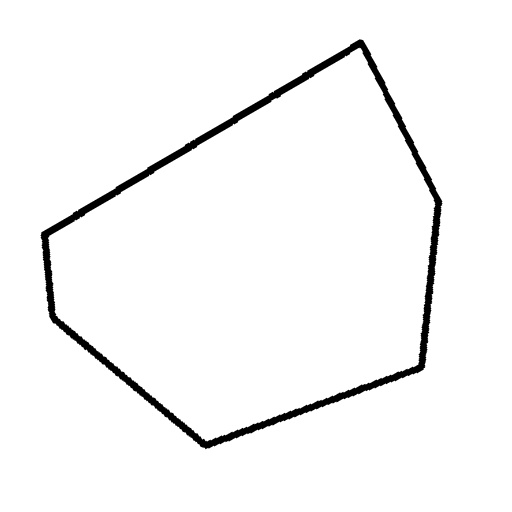
\includegraphics[width=.8\linewidth,frame]{img/experiment/dataset/5parcel.jpg}
                    \caption{Parcel image of the final datset.}
                    \label{fig:dataset-final-parcel}
                \end{minipage}%
                % \begin{minipage}{.5\textwidth}
                %     \centering
                %     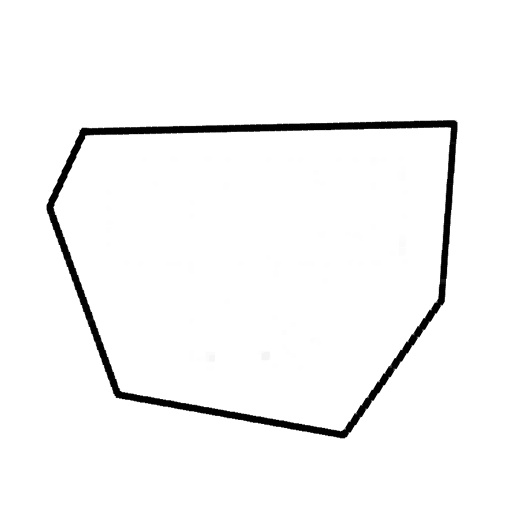
\includegraphics[width=.8\linewidth,frame]{img/experiment/dataset/4erode_img.jpg}
                %     \caption{Result when dilated image is eroded by stride of 5*5.}
                %     \label{fig:dataset-final-eroded}
                % \end{minipage}
            \end{figure}  
            Then we create a difference between the original image and the parcel giving us Floor plan without border line as in figure~\ref{fig:dataset-final-difference}, of which we first clear the doors and the furniture by doing dilation with 2*2 stride. Then we get the wall segmentation and then we erode the image with stride of 127*127 giving us the highly eroded image, i.e the wall segmentation would be changed to a very thick walled, i.e foot print of the floor planas in figure~\ref{fig:dataset-final-difference-eroded}.\\
            \begin{figure}[h]
                \centering
                \begin{minipage}{.5\textwidth}
                    \centering
                    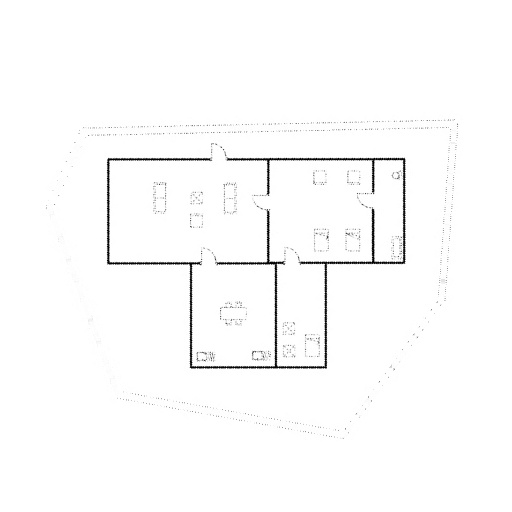
\includegraphics[width=.8\linewidth,frame]{img/experiment/dataset/6diff_img.jpg}
                    \caption{Difference of final dataset and parcel.}
                    \label{fig:dataset-final-difference}
                \end{minipage}%
                \hfill
                \begin{minipage}{.45\textwidth}
                    \centering
                    
\includegraphics[width=.8\linewidth,frame]{img/experiment/dataset/7erode_diff_img.jpg}
                    \caption{Result when difference image is dilated by stride of 2*2 then erroded by stride of 127*127.}
                    \label{fig:dataset-final-difference-eroded}
                \end{minipage}
            \end{figure}    
            \break    
            Then we dilate the image using stride of 125*125 giving us the floor plan's size as the size of original as shown in figure~\ref{fig:dataset-final-difference-dilated} then we thresholded the image to get exact black and white print as shown in figure~\ref{fig:dataset-final-difference-thresholded}.\\
            \begin{figure}[h]
                \centering
                \begin{minipage}{.45\textwidth}
                    \centering
                    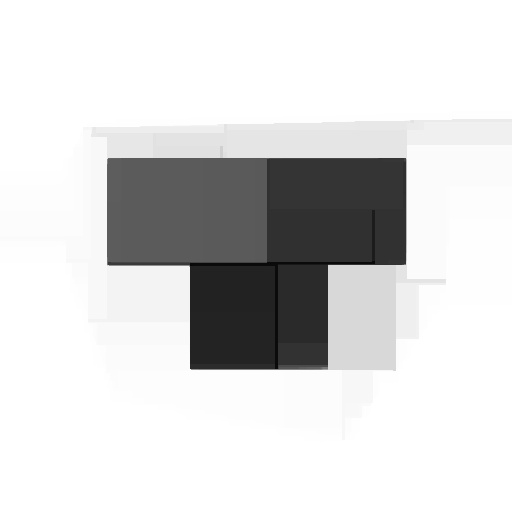
\includegraphics[width=.8\linewidth,frame]{img/experiment/dataset/8dilate_diff_img.jpg}
                    \caption{Dilated image is eroded back by stride of 125*125.}
                    \label{fig:dataset-final-difference-dilated}
                \end{minipage}%
                \hfill
                \begin{minipage}{.45\textwidth}
                    \centering
                    
\includegraphics[width=.8\linewidth,frame]{img/experiment/dataset/9footprint.jpg}
                    \caption{Dilated image is thresholded to get black and white print.}
                    \label{fig:dataset-final-difference-thresholded}
                \end{minipage}
            \end{figure}    
            \break 
            The plan is now the footprint which is then rotated clockwise 30 degree if required giving us final footprint shown in figure~\ref{fig:dataset-footprint}. Now we add the floor plan with the parcel and get the required footprint datasets shown in figure~\ref{fig:dataset-footprint-plus-parcel}. 
            \begin{figure}[h]
                \centering
                \begin{minipage}{.45\textwidth}
                    \centering
                    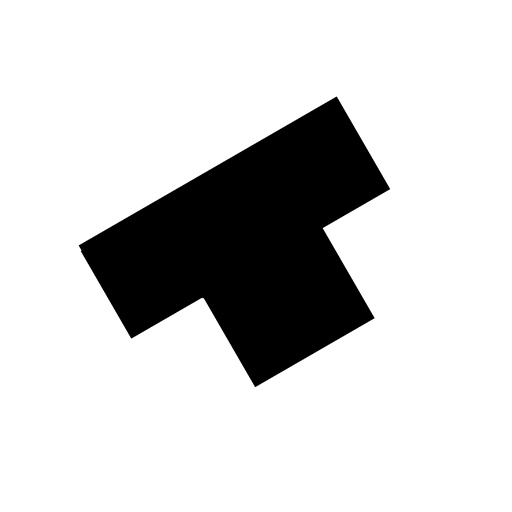
\includegraphics[width=.8\linewidth,frame]{img/experiment/dataset/10footprint_rotated.jpg}
                    \caption{Footprint}
                    \label{fig:dataset-footprint}
                \end{minipage}%
                \hfill
                \begin{minipage}{.45\textwidth}
                    \centering
                    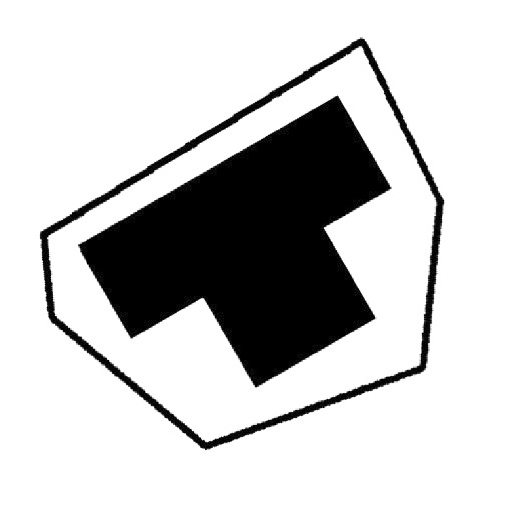
\includegraphics[width=.8\linewidth,frame]{img/experiment/dataset/11footprint_plus_parcel.jpg}
                    \caption{parcel added to footprint}
                    \label{fig:dataset-footprint-plus-parcel}
                \end{minipage}
            \end{figure}    
            \break 
            Since we needed paired image for translation from parcel to footprint, we concatenate the footprint datasets with the parcel and get footprint generation datasetsas shown in figure~\ref{fig:dataset-final-paired}.
            \begin{figure}[h]
                \centering
                    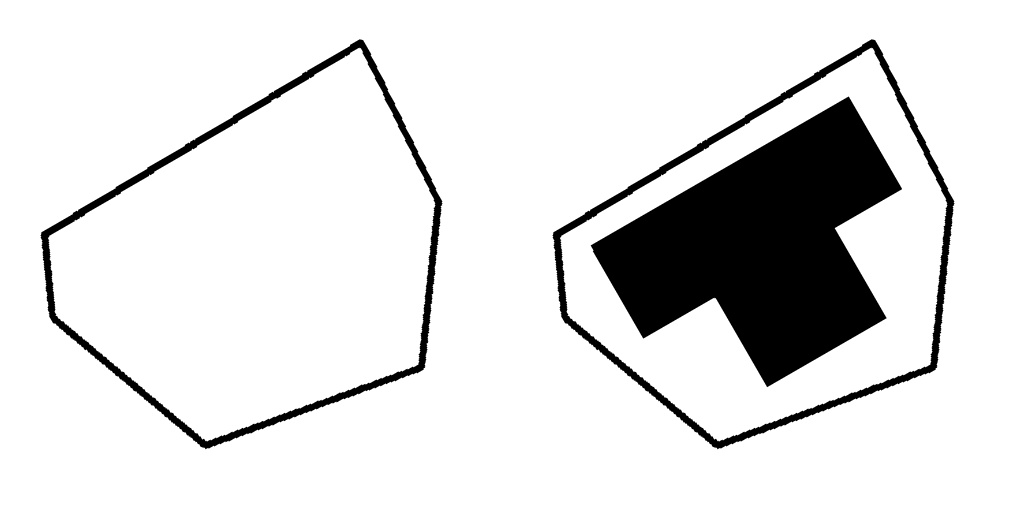
\includegraphics[width=.8\linewidth,frame]{img/experiment/dataset/12footprint_generation_dataset.jpg}
                    \caption{Paired image of parcel and required footprint.}
                    \label{fig:dataset-final-paired}
                
            \end{figure}    
            \break 
        {section:Parcel Generation from Cadestrial}
        For generation of Parcel from Cadestrial for deployment, we grab parcel area from cadestrial map by allowing the end user to manually draw over the map and select his land area and grab the corners of the selected area and place it over a plain white background giving us a parcel which is ready to go for further processing.\\
        Overall steps followed in these process are summarized below:
        First of all the selected image of cadestrial map is displayed in a new window and user is allowed to select corner points of his land area and the system draws the lines correspondingly as in figure~\ref{fig:cadestrial-drawn}.
        \begin{figure}
            \centering
            \begin{minipage}{.45\textwidth}
                \centering
                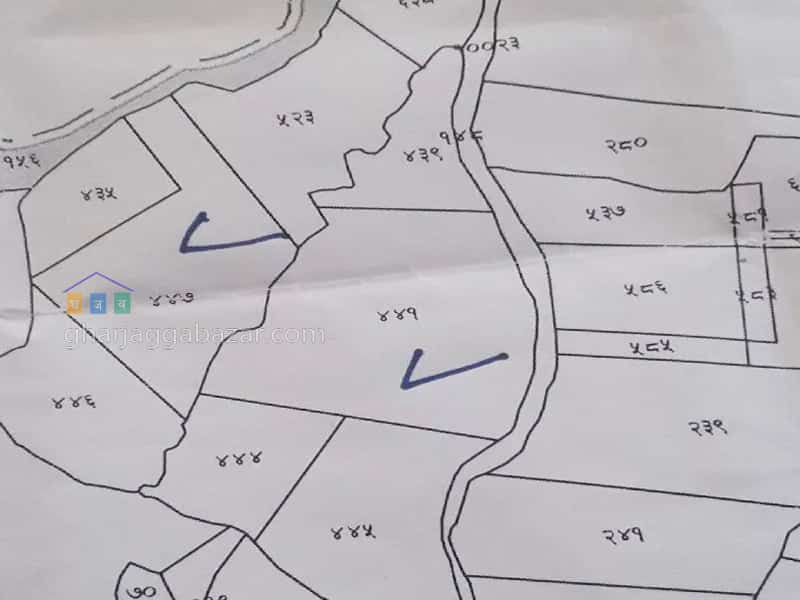
\includegraphics[width=.8\linewidth]{img/experiment/cadestrial_toparcel/naksa.jpg}
                \caption{Cadestrial map from Land Revenue Offices}
                \label{fig:cadestrial-orginal}
                
            \end{minipage}%
            \hfill
            \begin{minipage}{.45\textwidth}
                \centering
                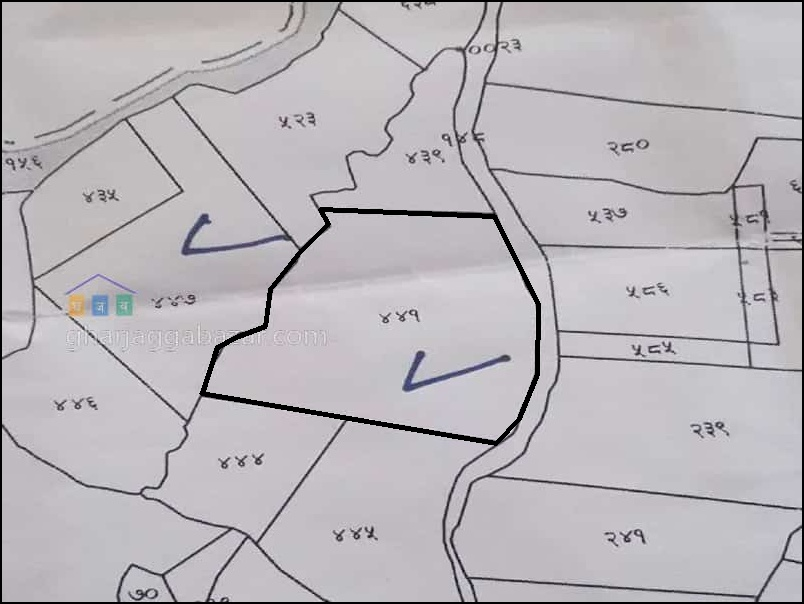
\includegraphics[width=.8\linewidth,frame]{img/experiment/cadestrial_toparcel/draw_over_naksa.jpg}
                \caption{Area of land drawn over cadestrial map.}
                \label{fig:cadestrial-drawn}
            \end{minipage}
        \end{figure}
        Then the corner points, i.e selected area were saved in an array. Then the coordinates of the corner points were brought toward origin by subtracting the minimum value of x coordinates from all x coordinates and minimum valur of y coordinated from all y coordinates, i.e (min(x),min(y)) from all the corner points. Then the result points were plotted in a new image giving us the land area of the user as in as in figure~\ref{fig:cadestrial-area}. Since the land area image was not ready for further processing by the system, it was further processed by placing it at center over a square background as in figure~\ref{fig:cadestrial-background} with white color and size 25\% bigger than the maximum side of the land area image giving us the parcel as in figure~\ref{fig:cadestrial-parcel} ready for further processing by the system. Then the parcel image is saved in remote after resizing it to the required size i.e 512*512.
        \begin{figure}
            \centering
            \begin{minipage}{.45\textwidth}
                \centering
                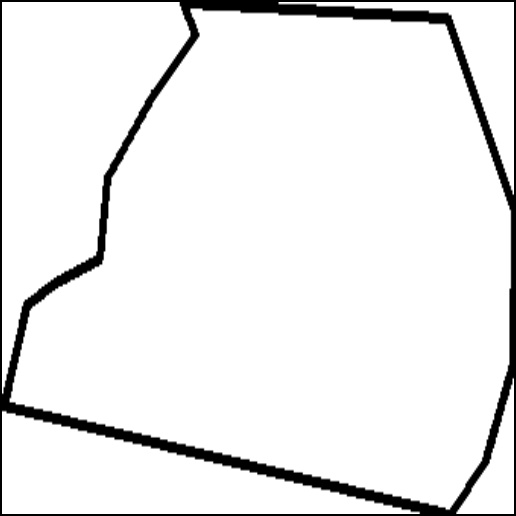
\includegraphics[width=.8\linewidth]{img/experiment/cadestrial_toparcel/area.jpg}
                \caption{Area of land selected by the user.}
                \label{fig:cadestrial-area}
            \end{minipage}%
            \hfill
            \begin{minipage}{.45\textwidth}
                \centering
                
\includegraphics[width=.8\linewidth,frame]{img/experiment/cadestrial_toparcel/bg.jpg}
                \caption{Background image for parcel}
                \label{fig:cadestrial-background}
            \end{minipage}
        \end{figure}
        \begin{figure}
            \centering
            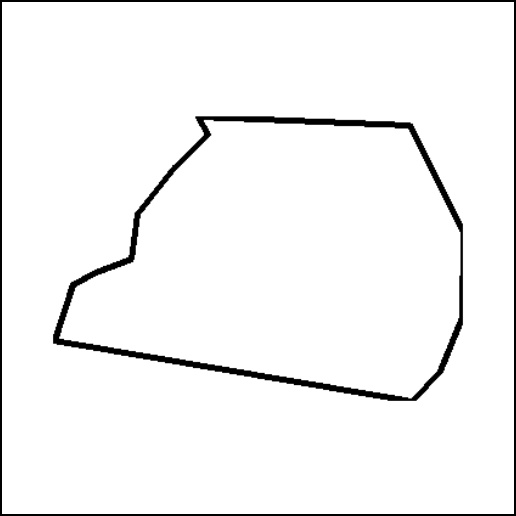
\includegraphics[width=.8\linewidth]{img/experiment/cadestrial_toparcel/parcel.jpg}
            \caption{parcel area formed by placing selected area over background.}
            \label{fig:cadestrial-parcel}
        \end{figure}
        \section{GAN Architectures}\label{section:gan-architecture}
            For the preparation of the GAN model, we need to first know the component of the GAN. A GAN model has three components. Namely:
            \begin{enumerate}[label=\alph*.]
                \item Generator  
                \item Discriminator 
                \item Loss Function
            \end{enumerate}
            Among these components, we mainly focus on the generator and discriminator. In case of the loss function, we have initially use the binary cross entropy, Mean Square Error, Mean Average Error.
    
            \subsection{Generator}\label{subsection:Generator}
                For generator, we have first need to constrained that, we are going to generate a new type of image using a image. So, we get condition from a image and then transfer the content of the image to generate another image. So, we need to have a generator model design in such a way that the input and output have the same dimension.  \\\\
                The same scenario is observed in the image segmentation in medical image in \cite{ronneberger2015u}. Also the similar architecture but the most advanced version of U-net i.e. Double U-net based architecture can also be used for the similar generation of image. So, here, we have two model for generation of image. 
            \subsection{Discriminator}\label{subsection:Discriminator}
                For discriminator, initially, Custom CNN model that takes two input images will be used as a discriminator and generate a model that gives an output 16*16 model will be used. \\\\
                Here, the discriminator model works in similar concept to classifier with classification classes real or fake. so, we have planned to prepare a model using Google Net pre-trained in image net datasets and change the top layer. The pre-trained model is used because it have already learn most generic features in lower layer (layer closes to the input layer) and also some high level features that using higher layer. So, we are going to use the concept of transfer learning for fast training and high accuracy. \\\\
                Not, only this, we can also have a u-net based architecture, that is build using encoder and decoder with skip connections. Here, the model can classify the whole image as real or fake and also, it can classify the each pixel as real or fake. So, we assume, this will be one of the power architecture for discriminator. Since, the discriminator is more powerful, so, the generator is also most powerful, since GAN is the competitive algorithm between generator and discriminator. \\\\
                So, in summary, we have 2 generator architecture and 3 discriminator architecture. And, in total we are going to have 6 GAN architecture for pix2pix image translation. 
    
            \subsection{GAN Architectures\label{subsection:ganarchitectures}}
            \begin{enumerate}[label=\alph*.]
                \item U-net Generator with Custom CNN Discriminator
                \item U-net Generator with Google net Discriminator
                \item U-net Generator with U-net based Discriminator as shown in \ref{Appendix: unetwithunet}
                \item Double U-net Generator with Custom CNN Discriminator
                \item Double U-net Generator with Google net Discriminator 
                \item Double U-net Generator with U-net based Discriminator
            \end{enumerate}
        \section{Condition for the Training}\label{section:conditionfortraining}
            \textbf{Datasets for training:} 
            The datasets for the training purpose is designed for 
            \begin{enumerate}[label=\alph*.]
                \item Parcel to Footprint\cite{footprint}
                \item Footprint to Room Split
                \begin{enumerate}[label=\roman*.]
                    \item 3 rooms
                    \item 4 rooms
                    \item 5 rooms
                \end{enumerate}
                \item Room Split to Furnished
            \end{enumerate}
           \begin{description}
               \item[No. of loop: ] For now, let's configure the no. of iteration for each model is 100,000.
               \item[GPU machine: ]  RTX 3060 with 3584 cuda cores and 12 GB RAM will be used for training purpose...
               \item[Training Time:] The training time can only be specify only after the we have successfully train the first model. Then, we can estimate the training time of each model using various architecture. And, then only we can compare between the result.
               \item[Val Loss:] The Val\_loss and Val\_acc will be tracked using the tensorboard, all the logs will be saved in logdir and shown using the val loss.
           \end{description}
            Then, after we observe the val loss and val accuracy, we can observe from where the model starts to over fit. 
            If the model over fit, it simply memories the style and content and the model will not be generic. So, we must observe where the model start over fitting. 
        \section{Model Comparision between different types of architecture}
            As we mention in \ref{section:gan-architecture}, there are 6 types of architecture we are going to implement in this project. So, we are going to compare between this model. So, for the comparison of different model, we need to fix some sort of data that is mentioned in \ref{section:conditionfortraining}. \\
            And, after the training is over, we will generate some datasets and then we will use inception score and FID score for the model evaluation. This score will be compare with each other model as well as with the ground truth image.
        \section{Generator}
            As mention in \ref{subsection:Generator}, We have two types of generator used to generate image. Namely: 
            \begin{enumerate}[label=\alph*.]
                \item U-net Generator
                \item Double U-net Generator
            \end{enumerate}
            \subsection{U-net Generator}
                The basic architecture of U-net Generator is also shown in figure \ref{fig:Architecture of the generator}. The detail summary of the architecture is given below: 
                {\scriptsize
                \begin{verbatim}
    Model: "U-net Generator"
    __________________________________________________________________________________________________
    Layer (type)                    Output Shape         Param #     Connected to                     
    ==================================================================================================
    input_22 (InputLayer)           [(None, 256, 256, 1) 0                                            
    __________________________________________________________________________________________________
    conv2d_139 (Conv2D)             (None, 128, 128, 64) 1088        input_22[0][0]                   
    __________________________________________________________________________________________________
    conv2d_140 (Conv2D)             (None, 64, 64, 128)  131200      conv2d_139[0][0]                 
    __________________________________________________________________________________________________
    batch_normalization_115 (BatchN (None, 64, 64, 128)  512         conv2d_140[0][0]                 
    __________________________________________________________________________________________________
    conv2d_141 (Conv2D)             (None, 32, 32, 256)  524544      batch_normalization_115[0][0]    
    __________________________________________________________________________________________________
    batch_normalization_116 (BatchN (None, 32, 32, 256)  1024        conv2d_141[0][0]                 
    __________________________________________________________________________________________________
    conv2d_142 (Conv2D)             (None, 16, 16, 512)  2097664     batch_normalization_116[0][0]    
    __________________________________________________________________________________________________
    batch_normalization_117 (BatchN (None, 16, 16, 512)  2048        conv2d_142[0][0]                 
    __________________________________________________________________________________________________
    conv2d_143 (Conv2D)             (None, 8, 8, 512)    4194816     batch_normalization_117[0][0]    
    __________________________________________________________________________________________________
    batch_normalization_118 (BatchN (None, 8, 8, 512)    2048        conv2d_143[0][0]                 
    __________________________________________________________________________________________________
    conv2d_144 (Conv2D)             (None, 4, 4, 512)    4194816     batch_normalization_118[0][0]    
    __________________________________________________________________________________________________
    batch_normalization_119 (BatchN (None, 4, 4, 512)    2048        conv2d_144[0][0]                 
    __________________________________________________________________________________________________
    conv2d_145 (Conv2D)             (None, 2, 2, 512)    4194816     batch_normalization_119[0][0]    
    __________________________________________________________________________________________________
    batch_normalization_120 (BatchN (None, 2, 2, 512)    2048        conv2d_145[0][0]                 
    __________________________________________________________________________________________________
    up_sampling2d_57 (UpSampling2D) (None, 4, 4, 512)    0           batch_normalization_120[0][0]    
    __________________________________________________________________________________________________
    conv2d_146 (Conv2D)             (None, 4, 4, 512)    4194816     up_sampling2d_57[0][0]           
    __________________________________________________________________________________________________
    batch_normalization_121 (BatchN (None, 4, 4, 512)    2048        conv2d_146[0][0]                 
    __________________________________________________________________________________________________
    concatenate_55 (Concatenate)    (None, 4, 4, 1024)   0           batch_normalization_121[0][0]    
                                                                        batch_normalization_119[0][0]    
    __________________________________________________________________________________________________
    up_sampling2d_58 (UpSampling2D) (None, 8, 8, 1024)   0           concatenate_55[0][0]             
    __________________________________________________________________________________________________
    conv2d_147 (Conv2D)             (None, 8, 8, 512)    8389120     up_sampling2d_58[0][0]           
    __________________________________________________________________________________________________
    batch_normalization_122 (BatchN (None, 8, 8, 512)    2048        conv2d_147[0][0]                 
    __________________________________________________________________________________________________
    concatenate_56 (Concatenate)    (None, 8, 8, 1024)   0           batch_normalization_122[0][0]    
                                                                        batch_normalization_118[0][0]    
    __________________________________________________________________________________________________
    up_sampling2d_59 (UpSampling2D) (None, 16, 16, 1024) 0           concatenate_56[0][0]             
    __________________________________________________________________________________________________
    conv2d_148 (Conv2D)             (None, 16, 16, 512)  8389120     up_sampling2d_59[0][0]           
    __________________________________________________________________________________________________
    batch_normalization_123 (BatchN (None, 16, 16, 512)  2048        conv2d_148[0][0]                 
    __________________________________________________________________________________________________
    concatenate_57 (Concatenate)    (None, 16, 16, 1024) 0           batch_normalization_123[0][0]    
                                                                        batch_normalization_117[0][0]    
    __________________________________________________________________________________________________
    up_sampling2d_60 (UpSampling2D) (None, 32, 32, 1024) 0           concatenate_57[0][0]             
    __________________________________________________________________________________________________
    conv2d_149 (Conv2D)             (None, 32, 32, 256)  4194560     up_sampling2d_60[0][0]           
    __________________________________________________________________________________________________
    batch_normalization_124 (BatchN (None, 32, 32, 256)  1024        conv2d_149[0][0]                 
    __________________________________________________________________________________________________
    concatenate_58 (Concatenate)    (None, 32, 32, 512)  0           batch_normalization_124[0][0]    
                                                                        batch_normalization_116[0][0]    
    __________________________________________________________________________________________________
    up_sampling2d_61 (UpSampling2D) (None, 64, 64, 512)  0           concatenate_58[0][0]             
    __________________________________________________________________________________________________
    conv2d_150 (Conv2D)             (None, 64, 64, 128)  1048704     up_sampling2d_61[0][0]           
    __________________________________________________________________________________________________
    batch_normalization_125 (BatchN (None, 64, 64, 128)  512         conv2d_150[0][0]                 
    __________________________________________________________________________________________________
    concatenate_59 (Concatenate)    (None, 64, 64, 256)  0           batch_normalization_125[0][0]    
                                                                        batch_normalization_115[0][0]    
    __________________________________________________________________________________________________
    up_sampling2d_62 (UpSampling2D) (None, 128, 128, 256 0           concatenate_59[0][0]             
    __________________________________________________________________________________________________
    conv2d_151 (Conv2D)             (None, 128, 128, 64) 262208      up_sampling2d_62[0][0]           
    __________________________________________________________________________________________________
    batch_normalization_126 (BatchN (None, 128, 128, 64) 256         conv2d_151[0][0]                 
    __________________________________________________________________________________________________
    concatenate_60 (Concatenate)    (None, 128, 128, 128 0           batch_normalization_126[0][0]    
                                                                        conv2d_139[0][0]                 
    __________________________________________________________________________________________________
    up_sampling2d_63 (UpSampling2D) (None, 256, 256, 128 0           concatenate_60[0][0]             
    __________________________________________________________________________________________________
    conv2d_152 (Conv2D)             (None, 256, 256, 1)  2049        up_sampling2d_63[0][0]           
    ==================================================================================================
    Total params: 41,837,185
    Trainable params: 41,828,353
    Non-trainable params: 8,832
    __________________________________________________________________________________________________
                                \end{verbatim}}
            \subsection{Double U-net Generator}
                The basic architecture of Double U-net Architecture is given below: 
                \begin{figure}[h]
                    \centering
                    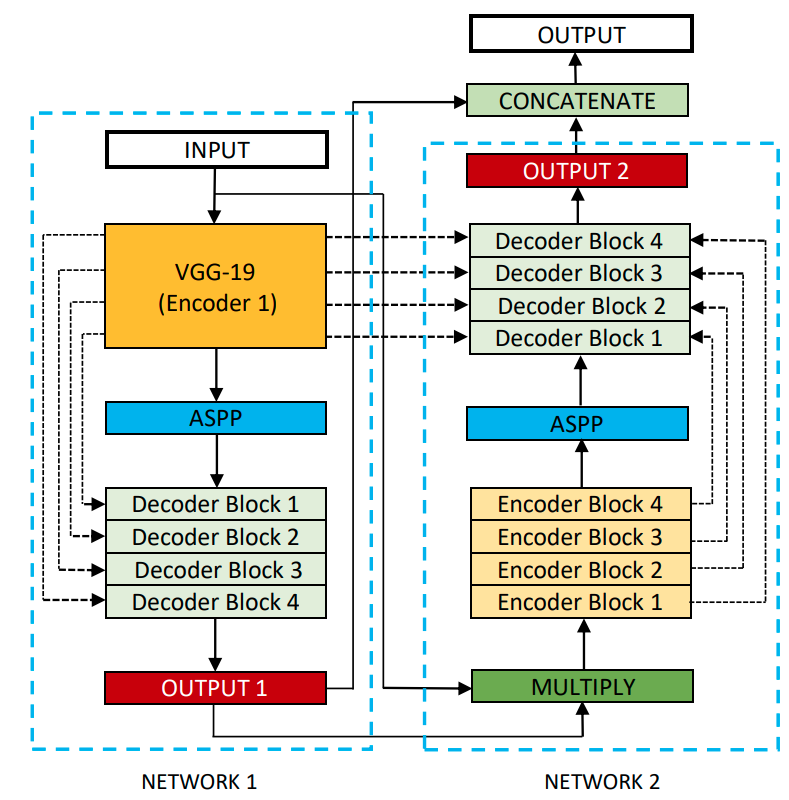
\includegraphics[width=.8\textwidth]{img/experiments/basicDoubleU-Net.png}
                    \caption{Double U-net Architecture}
                    \label{fig: Double U-net Architecture}
                \end{figure}   
                The detail summary of the architecture is given below:
                {\scriptsize
                \begin{verbatim}
    Model: "Double U-net Generator"
    __________________________________________________________________________________________________
    Layer (type)                    Output Shape         Param #     Connected to                     
    ==================================================================================================
    input_1 (InputLayer)            [(None, 512, 512, 3) 0                                            
    __________________________________________________________________________________________________
    block1_conv1 (Conv2D)           (None, 512, 512, 64) 1792        input_1[0][0]                    
    __________________________________________________________________________________________________
    block1_conv2 (Conv2D)           (None, 512, 512, 64) 36928       block1_conv1[0][0]               
    __________________________________________________________________________________________________
    block1_pool (MaxPooling2D)      (None, 256, 256, 64) 0           block1_conv2[0][0]               
    __________________________________________________________________________________________________
    block2_conv1 (Conv2D)           (None, 256, 256, 128 73856       block1_pool[0][0]                
    __________________________________________________________________________________________________
    block2_conv2 (Conv2D)           (None, 256, 256, 128 147584      block2_conv1[0][0]               
    __________________________________________________________________________________________________
    block2_pool (MaxPooling2D)      (None, 128, 128, 128 0           block2_conv2[0][0]               
    __________________________________________________________________________________________________
    block3_conv1 (Conv2D)           (None, 128, 128, 256 295168      block2_pool[0][0]                
    __________________________________________________________________________________________________
    block3_conv2 (Conv2D)           (None, 128, 128, 256 590080      block3_conv1[0][0]               
    __________________________________________________________________________________________________
    block3_conv3 (Conv2D)           (None, 128, 128, 256 590080      block3_conv2[0][0]               
    __________________________________________________________________________________________________
    block3_conv4 (Conv2D)           (None, 128, 128, 256 590080      block3_conv3[0][0]               
    __________________________________________________________________________________________________
    block3_pool (MaxPooling2D)      (None, 64, 64, 256)  0           block3_conv4[0][0]               
    __________________________________________________________________________________________________
    block4_conv1 (Conv2D)           (None, 64, 64, 512)  1180160     block3_pool[0][0]                
    __________________________________________________________________________________________________
    block4_conv2 (Conv2D)           (None, 64, 64, 512)  2359808     block4_conv1[0][0]               
    __________________________________________________________________________________________________
    block4_conv3 (Conv2D)           (None, 64, 64, 512)  2359808     block4_conv2[0][0]               
    __________________________________________________________________________________________________
    block4_conv4 (Conv2D)           (None, 64, 64, 512)  2359808     block4_conv3[0][0]               
    __________________________________________________________________________________________________
    block4_pool (MaxPooling2D)      (None, 32, 32, 512)  0           block4_conv4[0][0]               
    __________________________________________________________________________________________________
    block5_conv1 (Conv2D)           (None, 32, 32, 512)  2359808     block4_pool[0][0]                
    __________________________________________________________________________________________________
    block5_conv2 (Conv2D)           (None, 32, 32, 512)  2359808     block5_conv1[0][0]               
    __________________________________________________________________________________________________
    block5_conv3 (Conv2D)           (None, 32, 32, 512)  2359808     block5_conv2[0][0]               
    __________________________________________________________________________________________________
    block5_conv4 (Conv2D)           (None, 32, 32, 512)  2359808     block5_conv3[0][0]               
    __________________________________________________________________________________________________
    average_pooling2d (AveragePooli (None, 1, 1, 512)    0           block5_conv4[0][0]               
    __________________________________________________________________________________________________
    conv2d (Conv2D)                 (None, 1, 1, 64)     32832       average_pooling2d[0][0]          
    __________________________________________________________________________________________________
    batch_normalization (BatchNorma (None, 1, 1, 64)     256         conv2d[0][0]                     
    __________________________________________________________________________________________________
    conv2d_1 (Conv2D)               (None, 32, 32, 64)   32768       block5_conv4[0][0]               
    __________________________________________________________________________________________________
    conv2d_2 (Conv2D)               (None, 32, 32, 64)   294912      block5_conv4[0][0]               
    __________________________________________________________________________________________________
    conv2d_3 (Conv2D)               (None, 32, 32, 64)   294912      block5_conv4[0][0]               
    __________________________________________________________________________________________________
    conv2d_4 (Conv2D)               (None, 32, 32, 64)   294912      block5_conv4[0][0]               
    __________________________________________________________________________________________________
    activation (Activation)         (None, 1, 1, 64)     0           batch_normalization[0][0]        
    __________________________________________________________________________________________________
    batch_normalization_1 (BatchNor (None, 32, 32, 64)   256         conv2d_1[0][0]                   
    __________________________________________________________________________________________________
    batch_normalization_2 (BatchNor (None, 32, 32, 64)   256         conv2d_2[0][0]                   
    __________________________________________________________________________________________________
    batch_normalization_3 (BatchNor (None, 32, 32, 64)   256         conv2d_3[0][0]                   
    __________________________________________________________________________________________________
    batch_normalization_4 (BatchNor (None, 32, 32, 64)   256         conv2d_4[0][0]                   
    __________________________________________________________________________________________________
    up_sampling2d (UpSampling2D)    (None, 32, 32, 64)   0           activation[0][0]                 
    __________________________________________________________________________________________________
    activation_1 (Activation)       (None, 32, 32, 64)   0           batch_normalization_1[0][0]      
    __________________________________________________________________________________________________
    activation_2 (Activation)       (None, 32, 32, 64)   0           batch_normalization_2[0][0]      
    __________________________________________________________________________________________________
    activation_3 (Activation)       (None, 32, 32, 64)   0           batch_normalization_3[0][0]      
    __________________________________________________________________________________________________
    activation_4 (Activation)       (None, 32, 32, 64)   0           batch_normalization_4[0][0]      
    __________________________________________________________________________________________________
    concatenate (Concatenate)       (None, 32, 32, 320)  0           up_sampling2d[0][0]              
                                                                        activation_1[0][0]               
                                                                        activation_2[0][0]               
                                                                        activation_3[0][0]               
                                                                        activation_4[0][0]               
    __________________________________________________________________________________________________
    conv2d_5 (Conv2D)               (None, 32, 32, 64)   20480       concatenate[0][0]                
    __________________________________________________________________________________________________
    batch_normalization_5 (BatchNor (None, 32, 32, 64)   256         conv2d_5[0][0]                   
    __________________________________________________________________________________________________
    activation_5 (Activation)       (None, 32, 32, 64)   0           batch_normalization_5[0][0]      
    __________________________________________________________________________________________________
    up_sampling2d_1 (UpSampling2D)  (None, 64, 64, 64)   0           activation_5[0][0]               
    __________________________________________________________________________________________________
    concatenate_1 (Concatenate)     (None, 64, 64, 576)  0           up_sampling2d_1[0][0]            
                                                                        block4_conv4[0][0]               
    __________________________________________________________________________________________________
    conv2d_6 (Conv2D)               (None, 64, 64, 256)  1327360     concatenate_1[0][0]              
    __________________________________________________________________________________________________
    batch_normalization_6 (BatchNor (None, 64, 64, 256)  1024        conv2d_6[0][0]                   
    __________________________________________________________________________________________________
    activation_6 (Activation)       (None, 64, 64, 256)  0           batch_normalization_6[0][0]      
    __________________________________________________________________________________________________
    conv2d_7 (Conv2D)               (None, 64, 64, 256)  590080      activation_6[0][0]               
    __________________________________________________________________________________________________
    batch_normalization_7 (BatchNor (None, 64, 64, 256)  1024        conv2d_7[0][0]                   
    __________________________________________________________________________________________________
    activation_7 (Activation)       (None, 64, 64, 256)  0           batch_normalization_7[0][0]      
    __________________________________________________________________________________________________
    global_average_pooling2d (Globa (None, 256)          0           activation_7[0][0]               
    __________________________________________________________________________________________________
    reshape (Reshape)               (None, 1, 1, 256)    0           global_average_pooling2d[0][0]   
    __________________________________________________________________________________________________
    dense (Dense)                   (None, 1, 1, 32)     8192        reshape[0][0]                    
    __________________________________________________________________________________________________
    dense_1 (Dense)                 (None, 1, 1, 256)    8192        dense[0][0]                      
    __________________________________________________________________________________________________
    multiply (Multiply)             (None, 64, 64, 256)  0           activation_7[0][0]               
                                                                        dense_1[0][0]                    
    __________________________________________________________________________________________________
    up_sampling2d_2 (UpSampling2D)  (None, 128, 128, 256 0           multiply[0][0]                   
    __________________________________________________________________________________________________
    concatenate_2 (Concatenate)     (None, 128, 128, 512 0           up_sampling2d_2[0][0]            
                                                                        block3_conv4[0][0]               
    __________________________________________________________________________________________________
    conv2d_8 (Conv2D)               (None, 128, 128, 128 589952      concatenate_2[0][0]              
    __________________________________________________________________________________________________
    batch_normalization_8 (BatchNor (None, 128, 128, 128 512         conv2d_8[0][0]                   
    __________________________________________________________________________________________________
    activation_8 (Activation)       (None, 128, 128, 128 0           batch_normalization_8[0][0]      
    __________________________________________________________________________________________________
    conv2d_9 (Conv2D)               (None, 128, 128, 128 147584      activation_8[0][0]               
    __________________________________________________________________________________________________
    batch_normalization_9 (BatchNor (None, 128, 128, 128 512         conv2d_9[0][0]                   
    __________________________________________________________________________________________________
    activation_9 (Activation)       (None, 128, 128, 128 0           batch_normalization_9[0][0]      
    __________________________________________________________________________________________________
    global_average_pooling2d_1 (Glo (None, 128)          0           activation_9[0][0]               
    __________________________________________________________________________________________________
    reshape_1 (Reshape)             (None, 1, 1, 128)    0           global_average_pooling2d_1[0][0] 
    __________________________________________________________________________________________________
    dense_2 (Dense)                 (None, 1, 1, 16)     2048        reshape_1[0][0]                  
    __________________________________________________________________________________________________
    dense_3 (Dense)                 (None, 1, 1, 128)    2048        dense_2[0][0]                    
    __________________________________________________________________________________________________
    multiply_1 (Multiply)           (None, 128, 128, 128 0           activation_9[0][0]               
                                                                        dense_3[0][0]                    
    __________________________________________________________________________________________________
    up_sampling2d_3 (UpSampling2D)  (None, 256, 256, 128 0           multiply_1[0][0]                 
    __________________________________________________________________________________________________
    concatenate_3 (Concatenate)     (None, 256, 256, 256 0           up_sampling2d_3[0][0]            
                                                                        block2_conv2[0][0]               
    __________________________________________________________________________________________________
    conv2d_10 (Conv2D)              (None, 256, 256, 64) 147520      concatenate_3[0][0]              
    __________________________________________________________________________________________________
    batch_normalization_10 (BatchNo (None, 256, 256, 64) 256         conv2d_10[0][0]                  
    __________________________________________________________________________________________________
    activation_10 (Activation)      (None, 256, 256, 64) 0           batch_normalization_10[0][0]     
    __________________________________________________________________________________________________
    conv2d_11 (Conv2D)              (None, 256, 256, 64) 36928       activation_10[0][0]              
    __________________________________________________________________________________________________
    batch_normalization_11 (BatchNo (None, 256, 256, 64) 256         conv2d_11[0][0]                  
    __________________________________________________________________________________________________
    activation_11 (Activation)      (None, 256, 256, 64) 0           batch_normalization_11[0][0]     
    __________________________________________________________________________________________________
    global_average_pooling2d_2 (Glo (None, 64)           0           activation_11[0][0]              
    __________________________________________________________________________________________________
    reshape_2 (Reshape)             (None, 1, 1, 64)     0           global_average_pooling2d_2[0][0] 
    __________________________________________________________________________________________________
    dense_4 (Dense)                 (None, 1, 1, 8)      512         reshape_2[0][0]                  
    __________________________________________________________________________________________________
    dense_5 (Dense)                 (None, 1, 1, 64)     512         dense_4[0][0]                    
    __________________________________________________________________________________________________
    multiply_2 (Multiply)           (None, 256, 256, 64) 0           activation_11[0][0]              
                                                                        dense_5[0][0]                    
    __________________________________________________________________________________________________
    up_sampling2d_4 (UpSampling2D)  (None, 512, 512, 64) 0           multiply_2[0][0]                 
    __________________________________________________________________________________________________
    concatenate_4 (Concatenate)     (None, 512, 512, 128 0           up_sampling2d_4[0][0]            
                                                                        block1_conv2[0][0]               
    __________________________________________________________________________________________________
    conv2d_12 (Conv2D)              (None, 512, 512, 32) 36896       concatenate_4[0][0]              
    __________________________________________________________________________________________________
    batch_normalization_12 (BatchNo (None, 512, 512, 32) 128         conv2d_12[0][0]                  
    __________________________________________________________________________________________________
    activation_12 (Activation)      (None, 512, 512, 32) 0           batch_normalization_12[0][0]     
    __________________________________________________________________________________________________
    conv2d_13 (Conv2D)              (None, 512, 512, 32) 9248        activation_12[0][0]              
    __________________________________________________________________________________________________
    batch_normalization_13 (BatchNo (None, 512, 512, 32) 128         conv2d_13[0][0]                  
    __________________________________________________________________________________________________
    activation_13 (Activation)      (None, 512, 512, 32) 0           batch_normalization_13[0][0]     
    __________________________________________________________________________________________________
    global_average_pooling2d_3 (Glo (None, 32)           0           activation_13[0][0]              
    __________________________________________________________________________________________________
    reshape_3 (Reshape)             (None, 1, 1, 32)     0           global_average_pooling2d_3[0][0] 
    __________________________________________________________________________________________________
    dense_6 (Dense)                 (None, 1, 1, 4)      128         reshape_3[0][0]                  
    __________________________________________________________________________________________________
    dense_7 (Dense)                 (None, 1, 1, 32)     128         dense_6[0][0]                    
    __________________________________________________________________________________________________
    multiply_3 (Multiply)           (None, 512, 512, 32) 0           activation_13[0][0]              
                                                                        dense_7[0][0]                    
    __________________________________________________________________________________________________
    conv2d_14 (Conv2D)              (None, 512, 512, 1)  33          multiply_3[0][0]                 
    __________________________________________________________________________________________________
    activation_14 (Activation)      (None, 512, 512, 1)  0           conv2d_14[0][0]                  
    __________________________________________________________________________________________________
    tf.math.multiply (TFOpLambda)   (None, 512, 512, 3)  0           input_1[0][0]                    
                                                                        activation_14[0][0]              
    __________________________________________________________________________________________________
    conv2d_15 (Conv2D)              (None, 512, 512, 32) 896         tf.math.multiply[0][0]           
    __________________________________________________________________________________________________
    batch_normalization_14 (BatchNo (None, 512, 512, 32) 128         conv2d_15[0][0]                  
    __________________________________________________________________________________________________
    activation_15 (Activation)      (None, 512, 512, 32) 0           batch_normalization_14[0][0]     
    __________________________________________________________________________________________________
    conv2d_16 (Conv2D)              (None, 512, 512, 32) 9248        activation_15[0][0]              
    __________________________________________________________________________________________________
    batch_normalization_15 (BatchNo (None, 512, 512, 32) 128         conv2d_16[0][0]                  
    __________________________________________________________________________________________________
    activation_16 (Activation)      (None, 512, 512, 32) 0           batch_normalization_15[0][0]     
    __________________________________________________________________________________________________
    global_average_pooling2d_4 (Glo (None, 32)           0           activation_16[0][0]              
    __________________________________________________________________________________________________
    reshape_4 (Reshape)             (None, 1, 1, 32)     0           global_average_pooling2d_4[0][0] 
    __________________________________________________________________________________________________
    dense_8 (Dense)                 (None, 1, 1, 4)      128         reshape_4[0][0]                  
    __________________________________________________________________________________________________
    dense_9 (Dense)                 (None, 1, 1, 32)     128         dense_8[0][0]                    
    __________________________________________________________________________________________________
    multiply_4 (Multiply)           (None, 512, 512, 32) 0           activation_16[0][0]              
                                                                        dense_9[0][0]                    
    __________________________________________________________________________________________________
    max_pooling2d (MaxPooling2D)    (None, 256, 256, 32) 0           multiply_4[0][0]                 
    __________________________________________________________________________________________________
    conv2d_17 (Conv2D)              (None, 256, 256, 64) 18496       max_pooling2d[0][0]              
    __________________________________________________________________________________________________
    batch_normalization_16 (BatchNo (None, 256, 256, 64) 256         conv2d_17[0][0]                  
    __________________________________________________________________________________________________
    activation_17 (Activation)      (None, 256, 256, 64) 0           batch_normalization_16[0][0]     
    __________________________________________________________________________________________________
    conv2d_18 (Conv2D)              (None, 256, 256, 64) 36928       activation_17[0][0]              
    __________________________________________________________________________________________________
    batch_normalization_17 (BatchNo (None, 256, 256, 64) 256         conv2d_18[0][0]                  
    __________________________________________________________________________________________________
    activation_18 (Activation)      (None, 256, 256, 64) 0           batch_normalization_17[0][0]     
    __________________________________________________________________________________________________
    global_average_pooling2d_5 (Glo (None, 64)           0           activation_18[0][0]              
    __________________________________________________________________________________________________
    reshape_5 (Reshape)             (None, 1, 1, 64)     0           global_average_pooling2d_5[0][0] 
    __________________________________________________________________________________________________
    dense_10 (Dense)                (None, 1, 1, 8)      512         reshape_5[0][0]                  
    __________________________________________________________________________________________________
    dense_11 (Dense)                (None, 1, 1, 64)     512         dense_10[0][0]                   
    __________________________________________________________________________________________________
    multiply_5 (Multiply)           (None, 256, 256, 64) 0           activation_18[0][0]              
                                                                        dense_11[0][0]                   
    __________________________________________________________________________________________________
    max_pooling2d_1 (MaxPooling2D)  (None, 128, 128, 64) 0           multiply_5[0][0]                 
    __________________________________________________________________________________________________
    conv2d_19 (Conv2D)              (None, 128, 128, 128 73856       max_pooling2d_1[0][0]            
    __________________________________________________________________________________________________
    batch_normalization_18 (BatchNo (None, 128, 128, 128 512         conv2d_19[0][0]                  
    __________________________________________________________________________________________________
    activation_19 (Activation)      (None, 128, 128, 128 0           batch_normalization_18[0][0]     
    __________________________________________________________________________________________________
    conv2d_20 (Conv2D)              (None, 128, 128, 128 147584      activation_19[0][0]              
    __________________________________________________________________________________________________
    batch_normalization_19 (BatchNo (None, 128, 128, 128 512         conv2d_20[0][0]                  
    __________________________________________________________________________________________________
    activation_20 (Activation)      (None, 128, 128, 128 0           batch_normalization_19[0][0]     
    __________________________________________________________________________________________________
    global_average_pooling2d_6 (Glo (None, 128)          0           activation_20[0][0]              
    __________________________________________________________________________________________________
    reshape_6 (Reshape)             (None, 1, 1, 128)    0           global_average_pooling2d_6[0][0] 
    __________________________________________________________________________________________________
    dense_12 (Dense)                (None, 1, 1, 16)     2048        reshape_6[0][0]                  
    __________________________________________________________________________________________________
    dense_13 (Dense)                (None, 1, 1, 128)    2048        dense_12[0][0]                   
    __________________________________________________________________________________________________
    multiply_6 (Multiply)           (None, 128, 128, 128 0           activation_20[0][0]              
                                                                        dense_13[0][0]                   
    __________________________________________________________________________________________________
    max_pooling2d_2 (MaxPooling2D)  (None, 64, 64, 128)  0           multiply_6[0][0]                 
    __________________________________________________________________________________________________
    conv2d_21 (Conv2D)              (None, 64, 64, 256)  295168      max_pooling2d_2[0][0]            
    __________________________________________________________________________________________________
    batch_normalization_20 (BatchNo (None, 64, 64, 256)  1024        conv2d_21[0][0]                  
    __________________________________________________________________________________________________
    activation_21 (Activation)      (None, 64, 64, 256)  0           batch_normalization_20[0][0]     
    __________________________________________________________________________________________________
    conv2d_22 (Conv2D)              (None, 64, 64, 256)  590080      activation_21[0][0]              
    __________________________________________________________________________________________________
    batch_normalization_21 (BatchNo (None, 64, 64, 256)  1024        conv2d_22[0][0]                  
    __________________________________________________________________________________________________
    activation_22 (Activation)      (None, 64, 64, 256)  0           batch_normalization_21[0][0]     
    __________________________________________________________________________________________________
    global_average_pooling2d_7 (Glo (None, 256)          0           activation_22[0][0]              
    __________________________________________________________________________________________________
    reshape_7 (Reshape)             (None, 1, 1, 256)    0           global_average_pooling2d_7[0][0] 
    __________________________________________________________________________________________________
    dense_14 (Dense)                (None, 1, 1, 32)     8192        reshape_7[0][0]                  
    __________________________________________________________________________________________________
    dense_15 (Dense)                (None, 1, 1, 256)    8192        dense_14[0][0]                   
    __________________________________________________________________________________________________
    multiply_7 (Multiply)           (None, 64, 64, 256)  0           activation_22[0][0]              
                                                                        dense_15[0][0]                   
    __________________________________________________________________________________________________
    max_pooling2d_3 (MaxPooling2D)  (None, 32, 32, 256)  0           multiply_7[0][0]                 
    __________________________________________________________________________________________________
    average_pooling2d_1 (AveragePoo (None, 1, 1, 256)    0           max_pooling2d_3[0][0]            
    __________________________________________________________________________________________________
    conv2d_23 (Conv2D)              (None, 1, 1, 64)     16448       average_pooling2d_1[0][0]        
    __________________________________________________________________________________________________
    batch_normalization_22 (BatchNo (None, 1, 1, 64)     256         conv2d_23[0][0]                  
    __________________________________________________________________________________________________
    conv2d_24 (Conv2D)              (None, 32, 32, 64)   16384       max_pooling2d_3[0][0]            
    __________________________________________________________________________________________________
    conv2d_25 (Conv2D)              (None, 32, 32, 64)   147456      max_pooling2d_3[0][0]            
    __________________________________________________________________________________________________
    conv2d_26 (Conv2D)              (None, 32, 32, 64)   147456      max_pooling2d_3[0][0]            
    __________________________________________________________________________________________________
    conv2d_27 (Conv2D)              (None, 32, 32, 64)   147456      max_pooling2d_3[0][0]            
    __________________________________________________________________________________________________
    activation_23 (Activation)      (None, 1, 1, 64)     0           batch_normalization_22[0][0]     
    __________________________________________________________________________________________________
    batch_normalization_23 (BatchNo (None, 32, 32, 64)   256         conv2d_24[0][0]                  
    __________________________________________________________________________________________________
    batch_normalization_24 (BatchNo (None, 32, 32, 64)   256         conv2d_25[0][0]                  
    __________________________________________________________________________________________________
    batch_normalization_25 (BatchNo (None, 32, 32, 64)   256         conv2d_26[0][0]                  
    __________________________________________________________________________________________________
    batch_normalization_26 (BatchNo (None, 32, 32, 64)   256         conv2d_27[0][0]                  
    __________________________________________________________________________________________________
    up_sampling2d_5 (UpSampling2D)  (None, 32, 32, 64)   0           activation_23[0][0]              
    __________________________________________________________________________________________________
    activation_24 (Activation)      (None, 32, 32, 64)   0           batch_normalization_23[0][0]     
    __________________________________________________________________________________________________
    activation_25 (Activation)      (None, 32, 32, 64)   0           batch_normalization_24[0][0]     
    __________________________________________________________________________________________________
    activation_26 (Activation)      (None, 32, 32, 64)   0           batch_normalization_25[0][0]     
    __________________________________________________________________________________________________
    activation_27 (Activation)      (None, 32, 32, 64)   0           batch_normalization_26[0][0]     
    __________________________________________________________________________________________________
    concatenate_5 (Concatenate)     (None, 32, 32, 320)  0           up_sampling2d_5[0][0]            
                                                                        activation_24[0][0]              
                                                                        activation_25[0][0]              
                                                                        activation_26[0][0]              
                                                                        activation_27[0][0]              
    __________________________________________________________________________________________________
    conv2d_28 (Conv2D)              (None, 32, 32, 64)   20480       concatenate_5[0][0]              
    __________________________________________________________________________________________________
    batch_normalization_27 (BatchNo (None, 32, 32, 64)   256         conv2d_28[0][0]                  
    __________________________________________________________________________________________________
    activation_28 (Activation)      (None, 32, 32, 64)   0           batch_normalization_27[0][0]     
    __________________________________________________________________________________________________
    up_sampling2d_6 (UpSampling2D)  (None, 64, 64, 64)   0           activation_28[0][0]              
    __________________________________________________________________________________________________
    concatenate_6 (Concatenate)     (None, 64, 64, 832)  0           up_sampling2d_6[0][0]            
                                                                        block4_conv4[0][0]               
                                                                        multiply_7[0][0]                 
    __________________________________________________________________________________________________
    conv2d_29 (Conv2D)              (None, 64, 64, 256)  1917184     concatenate_6[0][0]              
    __________________________________________________________________________________________________
    batch_normalization_28 (BatchNo (None, 64, 64, 256)  1024        conv2d_29[0][0]                  
    __________________________________________________________________________________________________
    activation_29 (Activation)      (None, 64, 64, 256)  0           batch_normalization_28[0][0]     
    __________________________________________________________________________________________________
    conv2d_30 (Conv2D)              (None, 64, 64, 256)  590080      activation_29[0][0]              
    __________________________________________________________________________________________________
    batch_normalization_29 (BatchNo (None, 64, 64, 256)  1024        conv2d_30[0][0]                  
    __________________________________________________________________________________________________
    activation_30 (Activation)      (None, 64, 64, 256)  0           batch_normalization_29[0][0]     
    __________________________________________________________________________________________________
    global_average_pooling2d_8 (Glo (None, 256)          0           activation_30[0][0]              
    __________________________________________________________________________________________________
    reshape_8 (Reshape)             (None, 1, 1, 256)    0           global_average_pooling2d_8[0][0] 
    __________________________________________________________________________________________________
    dense_16 (Dense)                (None, 1, 1, 32)     8192        reshape_8[0][0]                  
    __________________________________________________________________________________________________
    dense_17 (Dense)                (None, 1, 1, 256)    8192        dense_16[0][0]                   
    __________________________________________________________________________________________________
    multiply_8 (Multiply)           (None, 64, 64, 256)  0           activation_30[0][0]              
                                                                        dense_17[0][0]                   
    __________________________________________________________________________________________________
    up_sampling2d_7 (UpSampling2D)  (None, 128, 128, 256 0           multiply_8[0][0]                 
    __________________________________________________________________________________________________
    concatenate_7 (Concatenate)     (None, 128, 128, 640 0           up_sampling2d_7[0][0]            
                                                                        block3_conv4[0][0]               
                                                                        multiply_6[0][0]                 
    __________________________________________________________________________________________________
    conv2d_31 (Conv2D)              (None, 128, 128, 128 737408      concatenate_7[0][0]              
    __________________________________________________________________________________________________
    batch_normalization_30 (BatchNo (None, 128, 128, 128 512         conv2d_31[0][0]                  
    __________________________________________________________________________________________________
    activation_31 (Activation)      (None, 128, 128, 128 0           batch_normalization_30[0][0]     
    __________________________________________________________________________________________________
    conv2d_32 (Conv2D)              (None, 128, 128, 128 147584      activation_31[0][0]              
    __________________________________________________________________________________________________
    batch_normalization_31 (BatchNo (None, 128, 128, 128 512         conv2d_32[0][0]                  
    __________________________________________________________________________________________________
    activation_32 (Activation)      (None, 128, 128, 128 0           batch_normalization_31[0][0]     
    __________________________________________________________________________________________________
    global_average_pooling2d_9 (Glo (None, 128)          0           activation_32[0][0]              
    __________________________________________________________________________________________________
    reshape_9 (Reshape)             (None, 1, 1, 128)    0           global_average_pooling2d_9[0][0] 
    __________________________________________________________________________________________________
    dense_18 (Dense)                (None, 1, 1, 16)     2048        reshape_9[0][0]                  
    __________________________________________________________________________________________________
    dense_19 (Dense)                (None, 1, 1, 128)    2048        dense_18[0][0]                   
    __________________________________________________________________________________________________
    multiply_9 (Multiply)           (None, 128, 128, 128 0           activation_32[0][0]              
                                                                        dense_19[0][0]                   
    __________________________________________________________________________________________________
    up_sampling2d_8 (UpSampling2D)  (None, 256, 256, 128 0           multiply_9[0][0]                 
    __________________________________________________________________________________________________
    concatenate_8 (Concatenate)     (None, 256, 256, 320 0           up_sampling2d_8[0][0]            
                                                                        block2_conv2[0][0]               
                                                                        multiply_5[0][0]                 
    __________________________________________________________________________________________________
    conv2d_33 (Conv2D)              (None, 256, 256, 64) 184384      concatenate_8[0][0]              
    __________________________________________________________________________________________________
    batch_normalization_32 (BatchNo (None, 256, 256, 64) 256         conv2d_33[0][0]                  
    __________________________________________________________________________________________________
    activation_33 (Activation)      (None, 256, 256, 64) 0           batch_normalization_32[0][0]     
    __________________________________________________________________________________________________
    conv2d_34 (Conv2D)              (None, 256, 256, 64) 36928       activation_33[0][0]              
    __________________________________________________________________________________________________
    batch_normalization_33 (BatchNo (None, 256, 256, 64) 256         conv2d_34[0][0]                  
    __________________________________________________________________________________________________
    activation_34 (Activation)      (None, 256, 256, 64) 0           batch_normalization_33[0][0]     
    __________________________________________________________________________________________________
    global_average_pooling2d_10 (Gl (None, 64)           0           activation_34[0][0]              
    __________________________________________________________________________________________________
    reshape_10 (Reshape)            (None, 1, 1, 64)     0           global_average_pooling2d_10[0][0]
    __________________________________________________________________________________________________
    dense_20 (Dense)                (None, 1, 1, 8)      512         reshape_10[0][0]                 
    __________________________________________________________________________________________________
    dense_21 (Dense)                (None, 1, 1, 64)     512         dense_20[0][0]                   
    __________________________________________________________________________________________________
    multiply_10 (Multiply)          (None, 256, 256, 64) 0           activation_34[0][0]              
                                                                        dense_21[0][0]                   
    __________________________________________________________________________________________________
    up_sampling2d_9 (UpSampling2D)  (None, 512, 512, 64) 0           multiply_10[0][0]                
    __________________________________________________________________________________________________
    concatenate_9 (Concatenate)     (None, 512, 512, 160 0           up_sampling2d_9[0][0]            
                                                                        block1_conv2[0][0]               
                                                                        multiply_4[0][0]                 
    __________________________________________________________________________________________________
    conv2d_35 (Conv2D)              (None, 512, 512, 32) 46112       concatenate_9[0][0]              
    __________________________________________________________________________________________________
    batch_normalization_34 (BatchNo (None, 512, 512, 32) 128         conv2d_35[0][0]                  
    __________________________________________________________________________________________________
    activation_35 (Activation)      (None, 512, 512, 32) 0           batch_normalization_34[0][0]     
    __________________________________________________________________________________________________
    conv2d_36 (Conv2D)              (None, 512, 512, 32) 9248        activation_35[0][0]              
    __________________________________________________________________________________________________
    batch_normalization_35 (BatchNo (None, 512, 512, 32) 128         conv2d_36[0][0]                  
    __________________________________________________________________________________________________
    activation_36 (Activation)      (None, 512, 512, 32) 0           batch_normalization_35[0][0]     
    __________________________________________________________________________________________________
    global_average_pooling2d_11 (Gl (None, 32)           0           activation_36[0][0]              
    __________________________________________________________________________________________________
    reshape_11 (Reshape)            (None, 1, 1, 32)     0           global_average_pooling2d_11[0][0]
    __________________________________________________________________________________________________
    dense_22 (Dense)                (None, 1, 1, 4)      128         reshape_11[0][0]                 
    __________________________________________________________________________________________________
    dense_23 (Dense)                (None, 1, 1, 32)     128         dense_22[0][0]                   
    __________________________________________________________________________________________________
    multiply_11 (Multiply)          (None, 512, 512, 32) 0           activation_36[0][0]              
                                                                        dense_23[0][0]                   
    __________________________________________________________________________________________________
    conv2d_37 (Conv2D)              (None, 512, 512, 1)  33          multiply_11[0][0]                
    __________________________________________________________________________________________________
    activation_37 (Activation)      (None, 512, 512, 1)  0           conv2d_37[0][0]                  
    __________________________________________________________________________________________________
    concatenate_10 (Concatenate)    (None, 512, 512, 2)  0           activation_14[0][0]              
                                                                        activation_37[0][0]              
    ==================================================================================================
    Total params: 29,297,570
    Trainable params: 29,290,274
    Non-trainable params: 7,296
    __________________________________________________________________________________________________
                                \end{verbatim}
                }
        \section{Discriminator}
            As mention in \ref{subsection:Discriminator}, we have three types of discriminator to be used in pix2pix GAN. Namely: 
            \begin{enumerate}[label=\alph*.]
                \item Simple CNN 
                \item Google Net Inception V3
                \item U-net Generator
            \end{enumerate}
            \subsection{Simple CNN}
                The architecture of the basic CNN model for discriminator is shown in figure \ref{fig:Simple CNN Discriminator Model}. 
                \begin{figure}[h]
                    \centering
                    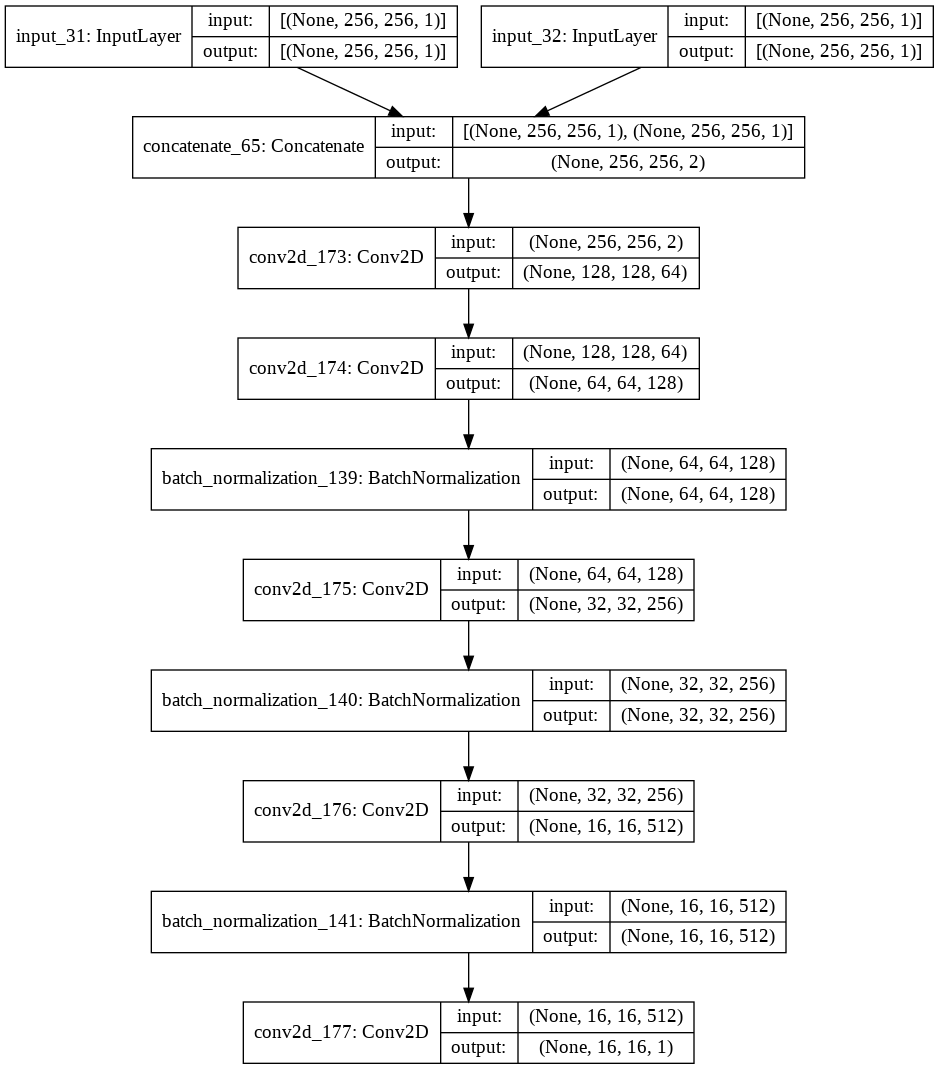
\includegraphics[width=.9\textwidth]{img/experiments/CNNDiscriminator_Model.png}
                    \caption{Simple CNN Discriminator Model}
                    \label{fig:Simple CNN Discriminator Model}
                \end{figure}
                
                The detail summary of the model is shown below:
                {\scriptsize
                \begin{verbatim}
    Model: "Simple CNN Discriminator
    __________________________________________________________________________________________________
    Layer (type)                    Output Shape         Param #     Connected to                     
    ==================================================================================================
    input_31 (InputLayer)           [(None, 256, 256, 1) 0                                            
    __________________________________________________________________________________________________
    input_32 (InputLayer)           [(None, 256, 256, 1) 0                                            
    __________________________________________________________________________________________________
    concatenate_65 (Concatenate)    (None, 256, 256, 2)  0           input_31[0][0]                   
                                                                        input_32[0][0]                   
    __________________________________________________________________________________________________
    conv2d_173 (Conv2D)             (None, 128, 128, 64) 2112        concatenate_65[0][0]             
    __________________________________________________________________________________________________
    conv2d_174 (Conv2D)             (None, 64, 64, 128)  131200      conv2d_173[0][0]                 
    __________________________________________________________________________________________________
    batch_normalization_139 (BatchN (None, 64, 64, 128)  512         conv2d_174[0][0]                 
    __________________________________________________________________________________________________
    conv2d_175 (Conv2D)             (None, 32, 32, 256)  524544      batch_normalization_139[0][0]    
    __________________________________________________________________________________________________
    batch_normalization_140 (BatchN (None, 32, 32, 256)  1024        conv2d_175[0][0]                 
    __________________________________________________________________________________________________
    conv2d_176 (Conv2D)             (None, 16, 16, 512)  2097664     batch_normalization_140[0][0]    
    __________________________________________________________________________________________________
    batch_normalization_141 (BatchN (None, 16, 16, 512)  2048        conv2d_176[0][0]                 
    __________________________________________________________________________________________________
    conv2d_177 (Conv2D)             (None, 16, 16, 1)    8193        batch_normalization_141[0][0]    
    ==================================================================================================
    Total params: 2,767,297
    Trainable params: 2,765,505
    Non-trainable params: 1,792
    __________________________________________________________________________________________________   
                \end{verbatim}}
            
        \section{Generator Metrics}
            Metrics on the basis of which we are going to test our final models are: 
            \begin{itemize}
                \item Inception score
                \item FID score
            \end{itemize}
        
            \subsection{Inception Score}
                For the development of better and logical evaluation metrics in the context of a Deep neural network involving generative models. Generative models need to be directly evaluated for the application they are intended for and as they are integrated into more complex systems, it'll be harder to discern their exact application aside from effectively capturing high-dimensional probability distributions thus necessitating high-quality evaluation metrics that are not specific to applications.The generative modeling community has developed various ad-hoc evaluative criteria. The Inception Score is one of these ad-hoc metrics that has gained popularity to evaluate the quality of generative models for images. \\
                Inception Score(IS) was shown to correlate well with human scoring of the realism of generated images from the CIFAR-10 dataset. The IS uses an Inception v3 Network pre-trained on ImageNet and calculates a statistic of the network’s outputs when applied to generated images. \\
                    \begin{equation}
                        {IS(G) = exp(\mathbb{E}_{x~p_g}D_{KL}(p(y|\mathsf{X}) \Vert p(y)))}
                    \end{equation}    
                    where ${\mathsf{X} ~ p_g}$ indicated that ${\mathsf{X}}$ is an image sampled from ${p_g}$, ${D_{KL}(p \Vert q)}$ is the KL-divergence between the distributions ${p}$ and ${q, p(y|\mathsf{X})}$ is the conditional class distribution and ${p(y) = \int_{\mathsf{X}}^{}p(y|\mathsf{X})p_g(\mathsf{X})}$ is the marginal class distribution. The exp in the expression is there to make the values easier to compare, so it will be ignored and we will use ${ln(IS(G))}$ without loss of generality.\\
                Considering the exponentiation new improved inception score is as follows:
                    \begin{equation}
                        {s(G) = \frac{1}{N}\sum^{N}_{i=1} D_{KL}(p(y|\mathsf{X}^{(i)} \Vert \hat{p}(y)))}
                    \end{equation}
            \subsection{FID Score}
                The Frechet Inception Distance score, or FID for short, is a metric that calculates the distance between feature vectors calculated for real and generated images.\\
                The score summarizes how similar the two groups are in terms of statistics on computer vision features of the raw images calculated using the inception v3 model used for image classification. Lower scores indicate the two groups of images are more similar, or have more similar statistics, with a perfect score being 0.0 indicating that the two groups of images are identical.\\    
                The FID score is used to evaluate the quality of images generated by generative adversarial networks, and lower scores have been shown to correlate well with higher-quality images. The FID score was proposed as an improvement over the existing Inception Score or IS.\\
                The FID score is calculated by first loading a pre-trained Inception v3 model.

                The output layer of the model is removed and the output is taken as the activations from the last pooling layer, a global spatial pooling layer.

                This output layer has 2,048 activations, therefore, each image is predicted as 2,048 activation features. This is called the coding vector or feature vector for the image.

                A 2,048 feature vector is then predicted for a collection of real images from the problem domain to provide a reference for how real images are represented. Feature vectors can then be calculated for synthetic images.

                The result will be two collections of 2,048 feature vectors for real and generated images.
                The FID score is then calculated using the following equation taken from the paper:
                \begin{equation}
                    {d^2 = {\Vert mu_1 – mu_2 \Vert}^2 + Tr(C_1 + C_2 – 2*\sqrt{C_1*C_2})}
                \end{equation}
                The score is referred to as ${d^2}$, showing that it is a distance and has squared units. The “${mu_1}$” and “${mu_2}$” refer to the feature-wise mean of the real and generated images, e.g. 2,048 element vectors where each element is the mean feature observed across the images.\\

        
        \section{Training Methodology}
            We have RTX 3060, and for proceeding the pix2pix GAN training using cuda cores and tensor cores, we need cuda toolkit and cuDNN. So, during installation we have two approach, 
            \begin{enumerate}[label=\alph*.]
                \item Using Docker Images
                \item Using miniConda as recommended by NVIDIA
            \end{enumerate}
            \subsection{Using Docker Images}
	            The docker image was created using the base image provided by NVIDIA/CUDA with images name nvidia/cuda:10.2-cudnn7-devel-ubuntu18.04. While creating the base image that has setup the environment for GAN. The TensorFlow with version 2.4.0 was installed. But, later we have found that the tensorflow latest version for linux is 2.2.0. So, we solve the problem using TensorFlow v2.2.0 instead of v2.5.0. And, we will be able to run the GAN model for training. 
            \subsection{Using miniConda as recommended by NVIDIA}
                As mention by Jeff Heaton in \cite{heaton_2021}, miniConda can be used to install python and tensorflow-gpu along with cuda and cudnn. And, we have also register the TensorFlow environment so that we can use it using Jupyter notebook.
        \section{TensorFlow Version Compatibility}
            The tensor flow version for 
            \begin{itemize}
                \item Google CoLab: 2.5
                \item Windows: 2.3
                \item Linux: 2.2
                \item Mac: 2.0
            \end{itemize}
            Here, the colab always has the highest version of tensorflow. Windows has 2.3 and linux has just 2.2 
    \section{Docker}
        \begin{itemize}%
            \item Docker is a platform for building, sharing, and running applications.
            \item Docker is a container engine.
            \item Docker is a tool for managing a containerized application.
        \end{itemize}

        \subsection{Dockerhub}
            \begin{itemize}%
                \item Dockerhub is a service for sharing and storing Docker images.
            \end{itemize}
            We have used the Docker image for nvidia/cuda:10.2-cudnn7-devel-ubuntu18.04 from the Dockerhub repository nvidia/cuda:10.2-cudnn7-devel-ubuntu18.04\cite{docker_hub_2021}.

        \subsection{Docker Image}
            \begin{itemize}%
                \item Docker Image is a bundle of files that defines an application.
            \end{itemize}
                The image for all project's model training wll be carried out on the basis of Dockerfile containing above dockerhub image as its base image.
                The layer wise description of the above mentioned image can be seen from nvidia/cuda:10.2-cudnn7-devel-ubuntu18.04\cite{docker_hub_2021}.

        \subsection{Dockerfile}
            \begin{itemize}%
                \item Dockerfile is a text document that contains all the instructions for building a Docker image.
                \item Dockerfile is a set of instructions that specify how to build a Docker image from a source code repository.
            \end{itemize}
            Docker file that we used to make the image for all project's model training is as follows:
\begin{verbatim}
FROM nvidia/cuda:10.2-cudnn7-devel-ubuntu18.04
ARG KERAS=2.4.0
ARG TENSORFLOW=2.5.0

ENV TZ=Asia/Kathmandu

RUN ln -snf /usr/share/zoneinfo/$TZ /etc/localtime && echo $TZ > /etc/timezone

RUN apt-get update

RUN apt-get install -y \
        python3 \
        curl \
        git \
        vim \
        python3-pip \
        python3-tk \
        wget \
        unzip

RUN pip3 install --upgrade pip

RUN pip3 --no-cache-dir install \
        tensorflow_gpu==${TENSORFLOW} \ 
        keras==${KERAS} \
        numpy \
        scipy \
        matplotlib \
        pandas \
        pillow
\end{verbatim}
            The docker base image created for this project can be found in base image gan 18\cite{dockerganbase}.
            Another base image was created using latest tensorflow version but without stating with the assumption that the Tensor flow of latest version for Linux will be installed.
\begin{verbatim}
FROM nvidia/cuda:10.2-cudnn7-devel-ubuntu18.04

ENV TZ=Asia/Kathmandu

RUN ln -snf /usr/share/zoneinfo/$TZ /etc/localtime && echo $TZ > /etc/timezone

RUN apt-get update

RUN apt-get install -y \
    python3 \
    curl \
    git \
    vim \
    python3-pip \
    python3-tk \
    wget \
    unzip

RUN pip3 install --upgrade pip

RUN pip3 --no-cache-dir install \
    tensorflow_gpu \ 
    keras \
    numpy \
    scipy \
    matplotlib \
    pandas \
    pillow
\end{verbatim}
            And, for the pix2pix GAN using unet and cnn the docker image is pubished at UnetAndCnn\cite{unetandcnn}. The Dockerfile for creating the docker image for unetandcnn is as follows: 
\begin{verbatim}
    FROM base_image_gan_18
    RUN apt update && apt install -y python3-pydot python-pydot-ng graphviz
    
    RUN pip3 install ipython args tqdm
    ADD . .
    RUN python3 download_datasets.py 
\end{verbatim} 
            This train can be begin using this docker image by running following script in bash. 
\begin{verbatim}
    sudo docker run bekojuniranjan/unetandcnn:v1 python3 src/run.py
\end{verbatim}
        \subsection{Docker Container}
            \begin{itemize}%
                \item Docker Container is a running instance of a Docker image.
            \end{itemize}
    
    \section{Activation Function}
        \subsection{Sigmoid Activation Function}
            Sigmoid function gives an ‘S’ shaped curve.The function maps any real value into another value between 0 and 1. Therefore, it is especially used for models where we have to predict the probability as an output.\\
            Equation:
            \begin{equation}
                f(x) = s = \frac{1}{1+e^{-x}}
            \end{equation}
            Derivative:
            \begin{equation}
                f'(x) = s *(1-s)
            \end{equation}
            Range: (0,1)
        \subsection{ReLU Activation Function}
        ReLU stands for rectified linear activation unit and is considered one of the few milestones in the deep learning revolution.\\
        Simple formula : 
        \begin{equation}
            f(x)=max(0,x)
        \end{equation}

        \subsection{Leaky ReLU Activation Function}
        Leaky ReLU function is an improved version of the ReLU activation function. As for the ReLU activation function, the gradient is 0 for all the values of inputs that are less than zero, which would deactivate the neurons in that region and may cause dying ReLU problem.\\\\
        Leaky ReLU is defined to address this problem. Instead of defining the ReLU activation function as 0 for negative values of inputs(x), we define it as an extremely small linear component of x. Here is the formula for this activation function\\
        \begin{equation}
            f(x)=max(0.01*x , x)
        \end{equation}
        Thus, it gives an output for negative values as well. \\

        \subsection{Softmax Activation Function}
        Softmax is not a traditional activation function. Other activation functions produce a single output for a single input. In contrast, softmax produces multiple outputs for an input array.  It not only maps our output to a [0,1] range but also maps each output in such a the output of softmax is therefore a probability distribution.\\\\
\noindent
        Equation: 
        \begin{equation}
            f(x) =  \frac{e^x_i}{(\sum_{j=\theta} e^x_i)}
        \end{equation}
        Probabilistic interpretation: 
        \begin{equation}
            S_j = P(y=j|x)
        \end{equation}
        Range: (0, 1)\\
        The softmax function is often used in the final layer of a neural network-based classifier.\\
        Softmax is used for multi-classification in logistic regression model. Softmax can be used to build neural networks models that can classify more than two classes instead of a binary class solution.\\

        \subsection{Tanh Activation Function}
        Tanh is also like logistic sigmoid but better. Tanh is also sigmoidal (s - shaped).\\
        Range: (-1, 1)\\\\
        The tanh function is mainly used classification between two classes.\\
     
    \noindent For our project, we have use leaky ReLU activation function among all of the above.
    While calculating, slope saturates when the input gets large in tanh, softmax and sigmoid function. In this case,
    ReLU activation function overcomes this problem. However, the slope of ReLU in the negative range is 0 so once a neuron gets negative, it’s unlikely for it to recover.
    This means neurons are not playing any role in discriminating the input and is essentially useless. Hence, to overcome all above
    mentioned problems, leaky ReLU is most convenient for use.
        
           
    \section{Loss Function}
        \subsection{Binary Cross Entropy}
            Binary cross entropy is a loss function that is used in binary classification tasks. These  tasks include answer to a  question with only two choices (yes or no, A or B, 0 or 1, left or right). Several independent such questions can be answered at the same time.\\
            The binary cross entropy is very convenient to train a model to solve many classification problems at the same time, if each classification can be reduced to a binary choice (i.e. yes or no, A or B, 0 or 1).\\
            Sigmoid function is only activation function compatible with  binary cross entropy.
            It can be explained as:
            \begin{equation}
                H_p(q) = -\frac{1}{N}\sum^N_{i=1}y_i.log(p(y_i)) + (1-y_i).log(1-p(y_i))
            \end{equation}
            Here, ${H_p(q)}$ is Binary Cross Entropy loss , x is the input , y is label (let labels be some color to points x:  label 1 is green and label 2 is red)/ output, ${p(y)}$ is probability of y being label 1, ${1-p(y)}$ is probability of y being label 2.Here, Binary cross entropy is the average of sum of log of probability of a point being red or green.
        \subsection{Categorical Cross Entropy}
            Categorical cross entropy is a loss function that is used in multi-class classification tasks. These are tasks where an example can only belong to one out of many possible categories, and the model must decide which one.\\
            Formally, it is designed to quantify the difference between two probability distributions.\\
            The categorical cross entropy is well suited to classification tasks, since one example can be considered to belong to a specific category with probability 1, and to other categories with probability 0.
            It can be explained as:
            \begin{equation}
                f(s)_i = \frac{e^{s_i}}{\sum^C_j e^{s_j}}
            \end{equation}
            \begin{equation}
                CE = - \sum^C_i t_i.log(f(s)_i)
            \end{equation}
            Here, ${t_i}$ is the groundtruth, i.e in the form of ${[0,0,0,1]}$, eg: for ${[cat, dog. horse, lion]}$ i.e multi class and ${f(s)_i}$ is result of softmax activation of multiple class eg: ${[0.2, 0.1, 0.3, 0.4]}$
            And, Higher the probability of the actual class in softmax result, lesser the loss and viceversa.

        \subsection{Mean Squared Error }
            The mean squared error (MSE) or mean squared deviation (MSD) of an estimator (of a procedure for estimating an unobserved quantity) measures the average of the squares of the errors that is, the average squared difference between the estimated values and the actual value. MSE is a risk function, corresponding to the expected value of the squared error loss. 
        \begin{equation}
            {MSE = \frac{1}{n}\sum^n_{i=1}(Y_i - \hat{Y_i})^2}
        \end{equation}
            Here, ${Y_i}$ is initial observed values while ${\hat{Y_i}}$ is the estimated or predicted value at any instance. MSE is the average of square of error between estimated and actual values.
        \subsection{Mean Absolute Error}
            mean absolute error (MAE) is a measure of errors between paired observations expressing the same phenomenon. Examples of Y versus X  include comparisons of predicted versus observed, subsequent time  versus initial time, and one technique of measurement versus an  alternative technique of measurement. MAE is calculated as:\\
        \begin{equation}
            {MAE = \frac{\sum^n_{i=1}|y_i - x_i|}{n}} = \frac{\sum^n_{i=1}|e_i|}{n}
        \end{equation}
        where, x is the observed values while y is the predicted values. MAE gives the average of sum of absolute error between observed values and predicted values at every instance.\\
        Descission boundary in classificaton task is large in comparison to regression. And MAE and MSE doesnot fix misclassification enough, but is a right loss for regression where distance between two values can be predicted is small. And from a probabilistic point of view, the binary cross-entropy arises as the natural cost function to use when we have a sigmoid function in the output layer of our network, and we want to maximize the likelihood of classifying the input data correctly. And categorical cross entropy is often used in case of multi class classifier.\\
        
    \section{Optimization Function}
        Optimization is the problem of finding a set of inputs to an objective function that results in a maximum or minimum function evaluation(Objective Function).\\
        Types of optimization function:
        \begin{itemize}
            \item Continuous Function Optimization
            \item Combinatorial Optimization problems
        \end{itemize}
        Continuous Function Optimization is encountered in problems where the objective function has real numbers as input arguments and output from the function.\\
        Combinatorial Optimization Problems is encountered in problems where the objective function has discrete value as input and output from the function.
        \subsection{Bracketing Algorithm}
            It's uses are: 
            \begin{enumerate}[label=\alph*.]
                \item Intended for optimization problems with only one input variable
                \item  Optima is known to exist within a specific range
                \item Specially used in finding the square roots of the number and solving a equation
                \item They assume single optima is present i.e. Unimodal objective function. 
            \end{enumerate}
        \subsection{Local Descent Algorithm}
            Local Descent Algorithm is used for optimization problem with more than one input variable and single global optima.\\ 
            Common Example is Line search Algorithm.\\
            It involves choosing a direction to move in the search space and then perform bracketing type search in a line or hyper plane in the choosen direction.\\
            It is computationally expensive to optimize each directional move in the search space.
        \subsection{First Order Algorithm}
            It uses the first derivative to choose the direction to move in the search space.\\
            Steps:
            \begin{enumerate}[label=\alph*.]
                \item First Calculate the gradient of the function.
                \item Follow the gradient in the opposite direction(e.g. downhill to the minimum for minimization problems)using a step size.(Learning Rate) 
                \item Step size is hyper parameter that control how far to move in the search space
                \item Small step size takes a longtime and can get stuck.
                \item Large step size results in zig-zagging or bouncing around search space.
            \end{enumerate} 
            \subsubsection{Gradient Descent}
                Gradient Descent Optimization Algorithm is popular often used as black box optimizer. It is most common way to optimize Neural Networks. Gradient descent is a way to minimize an objective function. Learning rate determines the size of the steps we take to reach local maxima. It follows the direction of slope downhill until we reach a valley.\\
                Variants of Gradient Descent are: 
                \begin{description}
                    \item [Batch Gradient Descent:] It computes gradient of the cost function with respect to the input in objective function for the entire training dataset.It is very slow and not used for datasets that does not fit in memory.It is guaranteed to converge to global minima for convex error surface.   
                    \item [Stochastic Gradient Descent:] It performs parameter update /tuning for each training examples. 
                    It solves problem that exists in batch gradient descent, performs redundant computation for large datasets. 
                    It updates with high variance that causes objective function to fluctuate heavily. 
                    It's fluctuation enables it to jump to new and potentially better local minima. 
                    \item [Mini batch gradient descent:] It updates for every mini-batches of a training examples. It reduces variance of parameters update and hence reduce fluctuation. It uses highly optimized matrix optimization.Its      common mini-batch size is 50-256.
                    \item [Momentum: ]It helps Stochastic Gradient Descent in the relevant direction and dampens oscillation. It is done by adding a fraction of the update vector of the past time.
                            \begin{equation}
                                v_t = \gamma v_{t-1} + \eta \nabla _\theta J(\theta)
                            \end{equation}
                            \begin{equation}
                                \theta = \theta - v_t
                            \end{equation}
                    \item [Adagrad:] It adapts the learning rate to the parameters. It performs larger updates for infrequent. It 
                    performs small updates for frequent parameters. 
                    Adagrad used different learning rate for every parameter at every time step.
                            \begin{equation}
                                \theta_t + 1,i = \theta_{t,i} - \frac{\eta}{\sqrt{G_{t,i}i + \epsilon .g_{t,i}}}
                            \end{equation}
                            \begin{equation}
                                {g_{t,i} = \nabla_{\theta_t}J(\theta_{t,i})}
                            \end{equation}
                    \item [Adadelta:]It is an extension of Adagrad.It reduces aggressive decreasing learning rate in Adagrad. Adagard accumulate all past squared gradients, but adadelta restrict the window of accumulated past gradients to some fixed sized w. The sum of gradients is recursively defined as a decaying average of all past squared gradients.
                    \begin{equation}
                        {E[g^2]_t = \gamma E[g^2]_{t-1} + (1- \gamma)g_t^2}
                    \end{equation} 
                    \item [Adam: ] It computes adaptive learning rate for each parameters. It has exponentially decaying average of past squared gradient. It includes momentum in adadelta or RMSprop. 
                    \begin{equation}
                        {\Delta w_i(t) = - \frac{\eta}{\sqrt{G_i(t)} + \epsilon}M_i(t)}
                    \end{equation}
                    \begin{equation}
                        {M_i(t) = \alpha M_i(t-1) + (1-\alpha)\frac{\delta L}{\delta w_i}(t)}
                    \end{equation}
                \end{description}
            \subsection{Second Order Algorithm}
                Example: Newton's Method, Secant Method, Quasi Newton Method\\\\\\
                Among, this all Optimization function, we choose Adam in our project for Optimization of Deep Neural Network as Adam includes momentum in Adadelta or RMSprop. and Adadelta is extension of Adagrad. So, in Adam Optimizer we have advantages of all Momentum, Adagrad and Adadelta. So, we choose Adam as optimization function. And, there is a wide practice of using Adam as optimization function in case of deep neural networks.
        
        % for seperate section optimization functions
        \section{3D Generation}
            For 3d Generation, one approach is 3D plotting of segmented image.
            For the plotting of 3D model, we used three python packages which are numpy, matplotlib and opencv using which we 3D plot the segmented image to 3D model. Here, first we get segmented image that contain segmentation of wall, door and window as shown in figure~\ref{fig:base-for-3d}.\\
            \begin{figure}[h]                 
                \centering                 
                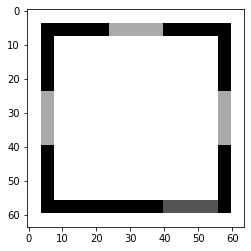
\includegraphics[width=.5\textwidth]{img/experiment/3d_generation/base-for-3d-generation.png}                 
                \caption{Segmented image required for 3D plotting.}                 
                \label{fig:base-for-3d}         
            \end{figure}
            \break
            Here, the white background represents floor, dark color band with gray level represents wall, band with gray level 85 represents window, gray level 170 represents door.
            The details is shown below in gray level format table~\ref{tab:graylevel}.\\
            \begin{table}[]
                \centering
                \caption{Gray level format in segmented image for 3D generation.}
                \label{tab:graylevel}
                \begin{tabular}{|c|c|}
                    \hline
                    \textbf{Component} & \textbf{Gray Level}\\
                    \hline
                    floor & 0\\
                    \hline
                    window & 85\\
                    \hline
                    door & 170\\
                    \hline
                    wall & 255\\
                    \hline
                \end{tabular}
            \end{table}
            \break
            But, while we generate the segmented image from the room split, we may not get exact gray level. So, for this we will use gray level slicing approaches as shown in figure~\ref{fig:gradable-slicing}.\\
            \begin{figure}[h]
                \centering
                \begin{minipage}{.45\textwidth}
                    \centering                 
                    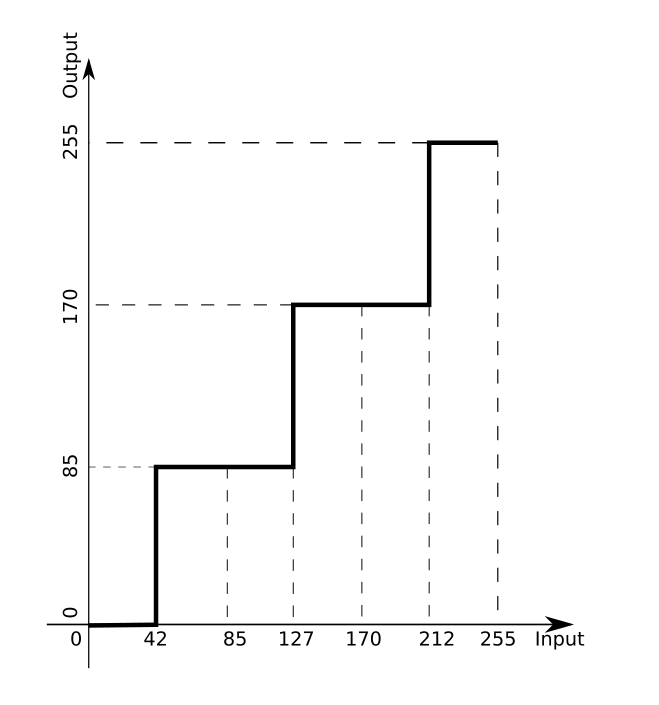
\includegraphics[width=1\textwidth]{img/experiment/3d_generation/gradable-slicing.png}                 
                    \caption{Graylevel slicing approach}                 
                    \label{fig:gradable-slicing}
                \end{minipage}%
                \hfill
                \begin{minipage}{.45\textwidth}
                    \centering                 
                    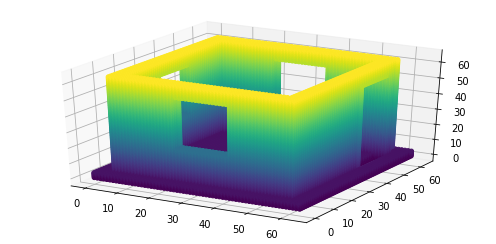
\includegraphics[width=1\textwidth]{img/experiment/3d_generation/3d-image.png}                 
                    \caption{3D Model Plotting}                 
                    \label{fig:3d-model} 
                \end{minipage}
            \end{figure}
            \break 
            Finally, we will replace the corresponding gray level with wall, floor, door, and window.  And the result will be display using the matplotlib 3d projection  Link of the colab  The output will be as shown in figure~\ref{fig:3d-model}.  
        
        \section{Convolution Layer}
            Convolution layer is one of the most important layer in deep neural network. It is used to extract features from the input image. It is also known as feature map.

            \begin{figure}[h]                 
                \centering                 
                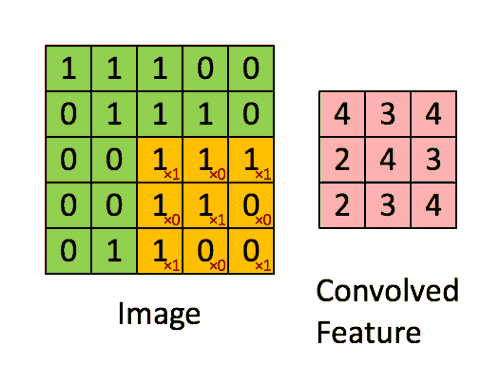
\includegraphics[width=.5\textwidth]{img/experiment/convolution.png}                 
                \caption{Convolutional layer convolved feature}                 
                \label{fig:Convolutional layer convolved feature}         
            \end{figure}
            \begin{equation}
                V(m,n) = \sum_{(k,l)\epsilon w}\sum z(k,l)y(m-k,n-l)
            \end{equation}
            Here, is a input image of 5*5*1 represented by green color, and a kernel of 3*3*1 represented by yellow color.\\ 
            The filter slides over the image to performs convolution operation and the result is shown in convolved feature in image.\\
            Here, the filter moves to the right with certain stride value till it parses the complete width. And, it hops down to the beginning of the image with the same stride value and repeat the process until the entire image is traversed.\\
            Here, the depth of the kernel is normally equal to the depth of the input image.
            \begin{figure}[h]                 
                \centering                 
                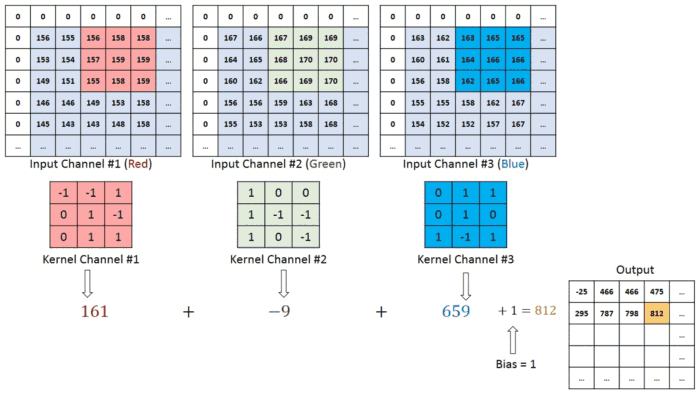
\includegraphics[width=1\textwidth]{img/experiment/convolution_of_three_channel_image.png}                 
                \caption{Convolution of three channel image}                 
                \label{fig:Convolution of three channel image}         
            \end{figure}
            Here, we have two types of operation. 
            \begin{itemize}
                \item \textbf{Same Padding} that performs the convolution in such a way that the output image has same dimension as input image. It first includes required padding in the input image.
                \item \textbf{Valid Padding} that perform the same operation without padding in input image. So, the output image dimension is less that that of input image.
            \end{itemize}

            \subsection{Same padding over valid padding}
                Let's take here a 3 x 3 image and 2 x 2 filter as shown in figure \ref{fig:Convolution using valid padding}. The value is not important for now. When we compute the convolution in the image with stride one, we visited four section of the image. One in the top-left, one in the top-right, one in the bottom-left and another in the bottom-right. Here, the center pixel is visited 4 times and the pixel at the corners are visited only once and remaining pixel are visited twice. So in valid padding, the pixel that locates at the center of the image is observed multiple time, but the pixel at the edge are not give much more importance. This means the information kept in the center gets more attention than the information on the edges. Hence, if the pixel at the edge is most important then it will miss the most important content in the image.
                \begin{figure}[h]                 
                    \centering                 
                    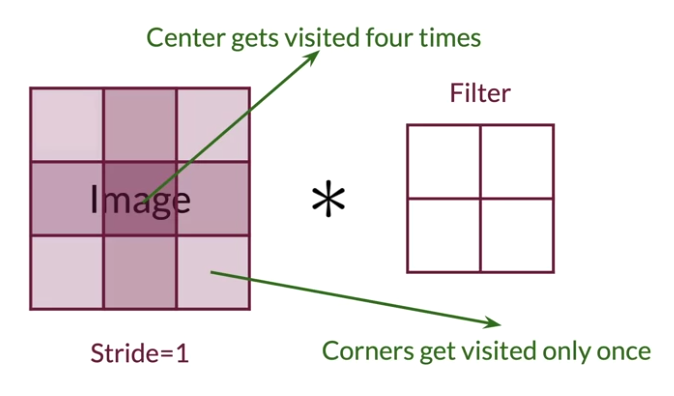
\includegraphics[width=.9\textwidth]{img/experiment/validpad.png}                 
                    \caption{Convolution using valid padding}                 
                    \label{fig:Convolution using valid padding}         
                \end{figure}
                So, we want to make sure that the filter puts equal emphasis across the entire image. To address this problem, we put a frame around the image so that the information appears at the center of this whole picture as in figure \ref{fig:Convolution using same padding} which is also known as padding. The padded value is usually zero. So, it is also called zero padding. Now, the filter scan the image along with the frame but this time the filter scans or visited each pixel of image equal no. of time. This is called same padding.
                \begin{figure}[h]                 
                    \centering                 
                    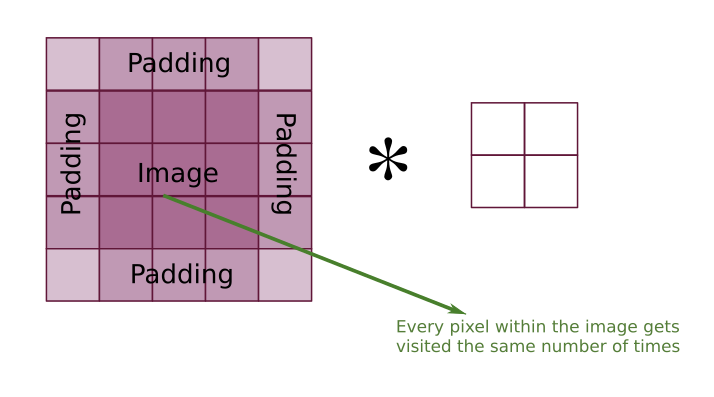
\includegraphics[width=.9\textwidth]{img/experiment/samepad.png}                 
                    \caption{Convolution using same padding}                 
                    \label{fig:Convolution using same padding}         
                \end{figure}
            \subsection{Convolution Layer follows Transpose Convolution}
                The Transpose Convolution layer is a learnable layer that takes the input image and convoluted it using a filter in such a way that the size of the input image increases. The difference between the transpose convolution and the up sampling layer is that up sampling has predefined method to up sample the image but the transpose convolution use the learnable parameter. 
                \begin{figure}[h]                 
                    \centering                 
                    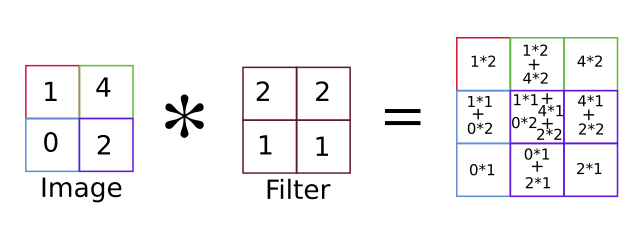
\includegraphics[width=.9\textwidth]{img/experiment/transConv2d.png}                 
                    \caption{Transpose Convolution}                 
                    \label{fig:Transpose Convolution}         
                \end{figure}
                Here, in the figure \ref{fig:Transpose Convolution}, the value of the filter are learned. But, there is an issue that the center pixel is visited four times and is influenced by all the pixels while the others are not. This raise an common issue called checkerboard issue as shown in figure \ref{fig:checkerboard Effect due to Transpose Convolution} This is the main disadvantage or defects of the transpose convolution layer.
                \begin{figure}[h]                 
                    \centering                 
                    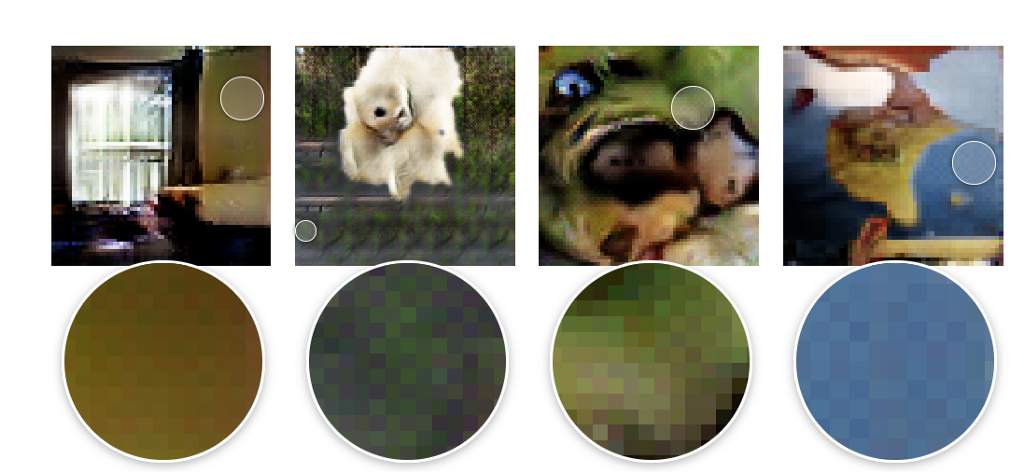
\includegraphics[width=.9\textwidth]{img/experiment/checkerboardeffect.png}                 
                    \caption{checkerboard Effect due to Transpose Convolution}                 
                    \label{fig:checkerboard Effect due to Transpose Convolution}         
                \end{figure}
        \section{Pooling Layer}
            It is similar to convolutional layer. It reduce the spatial size of the convolved feature. It helps to decrease the computational power required to process the data through dimensionality reduction. It is used for extracting dominant features.\\
            Types of Pooling:
            \begin{itemize}
                \item \textbf{Max Pooling}: It is used to extract the maximum value of the feature map.It also performs as Noise Suppressant.
                \item \textbf{Average Pooling} : It is used to extract the average value of the feature map.It simply performs dimensionality reduction.
            \end{itemize} 
            \begin{figure}[h]                 
                \centering                 
                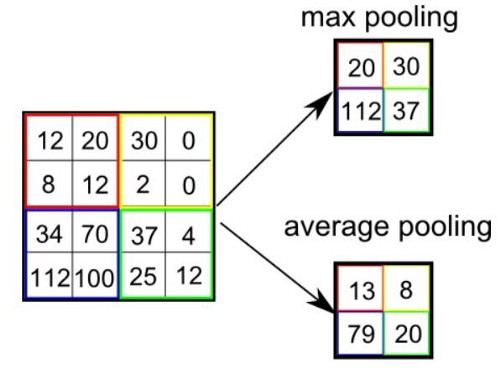
\includegraphics[width=.5\textwidth]{img/experiment/pooling_layers.png}                 
                \caption{Pooling layers}                 
                \label{fig:Pooling layers}         
            \end{figure}